\documentclass{article}
% Recommended, but optional, packages for figures and better typesetting:
\usepackage{microtype}
\usepackage{graphicx}
\usepackage{subfigure}
\newcommand{\theHalgorithm}{\arabic{algorithm}}
\usepackage{caption}
\usepackage{xspace}
\usepackage{pifont}
\usepackage{booktabs} % for professional tables
% hyperref makes hyperlinks in the resulting PDF.
% If your build breaks (sometimes temporarily if a hyperlink spans a page)
% please comment out the following usepackage line and replace
\usepackage{hyperref}
\usepackage{xcolor}
\usepackage{listings}
\usepackage{times}
\usepackage{latexsym}

\usepackage{algorithm}
\usepackage{algorithmic}

% For proper rendering and hyphenation of words containing Latin characters (including in bib files)
\usepackage[T1]{fontenc}
% For Vietnamese characters
% \usepackage[T5]{fontenc}
% See https://www.latex-project.org/help/documentation/encguide.pdf for other character sets

% This assumes your files are encoded as UTF8
\usepackage[utf8]{inputenc}
% Attempt to make hyperref and algorithmic work together better:



% Use the following line for the initial blind version submitted for review:
\usepackage[final]{acl}

% If accepted, instead use the following line for the camera-ready submission:

% For theorems and such
\usepackage{amsmath}
\usepackage{amssymb}
\usepackage{mathtools}
\usepackage{amsthm}
\usepackage{multirow}
\usepackage{graphicx}
\usepackage{lscape}
% if you use cleveref..
\usepackage[capitalize,noabbrev]{cleveref}
\newcommand{\xin}[1]{\textcolor{orange}{Xin: #1}}  % 
%%%%%%%%%%%%%%%%%%%%%%%%%%%%%%%%
% THEOREMS
%%%%%%%%%%%%%%%%%%%%%%%%%%%%%%%%
\theoremstyle{plain}
\newtheorem{theorem}{Theorem}[section]
\newtheorem{proposition}[theorem]{Proposition}
\newtheorem{lemma}[theorem]{Lemma}
\newtheorem{corollary}[theorem]{Corollary}
\theoremstyle{definition}
\newtheorem{definition}[theorem]{Definition}
\newtheorem{assumption}[theorem]{Assumption}
\theoremstyle{remark}
\newtheorem{remark}[theorem]{Remark}
\newcommand{\sysname}{\texttt{AgentSpec}\xspace}
% \newcommand{\sysnamew}{\texttt{SVDLLM-W}\xspace}
% \newcommand{\sysnamewl}{\texttt{SVDLLM-WL}\xspace}
\newcommand{\remaining}[1]{\textcolor{red}{Mark: #1}}

\definecolor{mygreen}{HTML}{009901}
\newcommand{\spup}[1]{\textcolor{mygreen}{#1}}
\newcommand{\spdown}[1]{\textcolor{red}{#1}}
\newcommand{\spone}[1]{\textcolor{gray}{#1}}
% Todonotes is useful during development; simply uncomment the next line
%    and comment out the line below the next line to turn off comments
%\usepackage[disable,textsize=tiny]{todonotes}
\usepackage[textsize=tiny]{todonotes}
\lstset{
  basicstyle=\ttfamily\small,
  columns=fullflexible,
  frame=single,
  breaklines=true,
  showstringspaces=false,
  keywordstyle=\color{blue},
  commentstyle=\spup,
  stringstyle=\color{blue},
}
\newcommand{\eeTable}{{
\begin{table*}[t]
\centering
\caption{Goodput (tokens/sec) of \sysname and baselines on four different agentic workloads with three different models. The best performance is marked in bold. The speedup is measured by comparing the goodput with the normal autoregressive decoding. The relative performance gain compared to the best-performing baseline is marked in green inside bracket.}
\label{tab:e2e_comparison}
\resizebox{0.95\linewidth}{!}{
\begin{tabular}{c|c|cc|cc|cc|cc}
\toprule
\textsc{Model} & \textsc{Method}
& \multicolumn{2}{c|}{Deep Research Agent}
& \multicolumn{2}{c|}{Code Generation Agent}
& \multicolumn{2}{c|}{GAIA}
& \multicolumn{2}{c}{SWE-Bench}\\
\cmidrule(lr){3-4}\cmidrule(lr){5-6}\cmidrule(lr){7-8}\cmidrule(lr){9-10}
& & Tokens/s & Speedup & Tokens/s & Speedup & Tokens/s & Speedup & Tokens/s & Speedup\\
\midrule

% ---------------- Qwen-3-8B ----------------
\multirow{5}{*}{\rotatebox[origin=c]{90}{\textbf{Qwen-3-8B}}} & Normal
& 617.41 & \spone{$\times$ 1.00}
& 636.09 & \spone{$\times$ 1.00}
& 501.27 & \spone{$\times$ 1.00}
& 652.44 & \spone{$\times$ 1.00} \\ \cmidrule{2-10}
         & EAGLE-3
& 605.14 & \spdown{$\times$ 0.98}
& 539.01 & \spdown{$\times$ 0.85}
& 468.22 & \spdown{$\times$ 0.93}
& 523.12 & \spdown{$\times$ 0.80} \\
         & NGram
& 509.62 & \spdown{$\times$ 0.83}
& 422.58 & \spdown{$\times$ 0.66}
& 308.27 & \spdown{$\times$ 0.61}
& 408.28 & \spdown{$\times$ 0.63} \\
         & SuffixDecoding
& 598.74 & \spdown{$\times$ 0.97}
& 579.21 & \spdown{$\times$ 0.91}
& 498.16 & \spdown{$\times$ 0.99}
& 556.64 & \spdown{$\times$ 0.85} \\ \cmidrule{2-10}
         & \sysname
& \textbf{661.43} \spup{($\uparrow 9\%$)}  & \spup{\textbf{$\times$ 1.07}}
& \textbf{828.10} \spup{($\uparrow 43\%$)} & \spup{\textbf{$\times$ 1.30}}
& \textbf{537.78} \spup{($\uparrow 8\%$)}  & \spup{\textbf{$\times$ 1.07}}
& \textbf{854.69} \spup{($\uparrow 42\%$)} & \spup{\textbf{$\times$ 1.31}} \\
\midrule

% ---------------- GPT-OSS-20B ----------------
\multirow{5}{*}{\rotatebox[origin=c]{90}{\textbf{GPT-OSS-20B}}} & Normal
& 201.43 & \spone{$\times$ 1.00}
& 289.26 & \spone{$\times$ 1.00}
& 247.67 & \spone{$\times$ 1.00}
& 351.22 & \spone{$\times$ 1.00} \\ \cmidrule{2-10}
            & EAGLE-3
& 125.71 & \spdown{$\times$ 0.62}
& 161.34 & \spdown{$\times$ 0.56}
& 112.16 & \spdown{$\times$ 0.45}
& 198.81 & \spdown{$\times$ 0.57} \\
            & NGram
& 158.91 & \spdown{$\times$ 0.79}
& 175.19 & \spdown{$\times$ 0.61}
& 109.22 & \spdown{$\times$ 0.44}
& 253.36 & \spdown{$\times$ 0.72} \\
            & SuffixDecoding
& 196.54 & \spdown{$\times$ 0.98}
& 295.85 & \spup{$\times$ 1.02}
& 187.79 & \spdown{$\times$ 0.76}
& 319.73 & \spdown{$\times$ 0.91} \\ \cmidrule{2-10}
            & \sysname
& \textbf{297.54} \spup{($\uparrow 51\%$)} & \spup{\textbf{$\times$ 1.48}}
& \textbf{584.43} \spup{($\uparrow 104\%$)} & \spup{\textbf{$\times$ 2.02}}
& \textbf{295.76} \spup{($\uparrow 57\%$)} & \spup{\textbf{$\times$ 1.19}}
& \textbf{595.20} \spup{($\uparrow 86\%$)} & \spup{\textbf{$\times$ 1.69}} \\
\midrule

% ---------------- DSK-8B ----------------
\multirow{5}{*}{\rotatebox[origin=c]{90}{\textbf{DSK-Distill-8B}}} & Normal
& 987.66  & \spone{$\times$ 1.00}
& 1230.28 & \spone{$\times$ 1.00}
& 823.39  & \spone{$\times$ 1.00}
& 1432.27 & \spone{$\times$ 1.00} \\ \cmidrule{2-10}
       & EAGLE-3
& 965.43  & \spdown{$\times$ 0.98}
& 1119.29 & \spdown{$\times$ 0.91}
& 864.43  & \spup{$\times$ 1.05}
& 1098.82 & \spdown{$\times$ 0.77} \\
       & NGram
& 752.66  & \spdown{$\times$ 0.76}
& 797.18  & \spdown{$\times$ 0.65}
& 725.29  & \spdown{$\times$ 0.88}
& 1014.47 & \spdown{$\times$ 0.71} \\
       & SuffixDecoding
& 995.14  & \spup{$\times$ 1.01}
& 1041.29 & \spdown{$\times$ 0.85}
& 820.09  & \spone{$\times$ 1.00}
& 1498.69 & \spup{$\times$ 1.05} \\ \cmidrule{2-10}
       & \sysname
& \textbf{1294.65} \spup{($\uparrow 30\%$)} & \spup{\textbf{$\times$ 1.31}}
& \textbf{1671.34} \spup{($\uparrow 49\%$)} & \spup{\textbf{$\times$ 1.36}}
& \textbf{924.47}  \spup{($\uparrow 7\%$)}  & \spup{\textbf{$\times$ 1.12}}
& \textbf{2281.87} \spup{($\uparrow 52\%$)} & \spup{\textbf{$\times$ 1.59}}\\
\bottomrule
\end{tabular}
}
\end{table*}
}}




% ================= Table: MiMo-7B USACO (Thpt + Spd) =================
\newcommand{\mimoTable}{{
\begin{table*}[ht]
\centering
\caption{Goodput (tokens/sec) of \sysname and baselines, including MTP, on MiMo-7B. The best performance is marked in bold. The speedup is measured by comparing the goodput with the normal autoregressive decoding. The relative performance gain compared to the best-performing baseline is marked in green inside bracket.}
\label{tab:mimo_usaco}
\resizebox{1\linewidth}{!}{
\begin{tabular}{c| c| cc cc cc cc cc}
\toprule
\textsc{Model} & \textsc{Method}
& \multicolumn{2}{c}{Code Gen.(Bronze)}
& \multicolumn{2}{c}{Code Gen.(Silver)}
& \multicolumn{2}{c}{Code Gen.(Gold)}
& \multicolumn{2}{c}{Code Gen.(Platinum)}
& \multicolumn{2}{c}{Code Gen.(All)} \\
\cmidrule(lr){3-4}\cmidrule(lr){5-6}\cmidrule(lr){7-8}\cmidrule(lr){9-10}\cmidrule(lr){11-12}
& & Tokens/s & Speedup & Tokens/s & Speedup & Tokens/s & Speedup & Tokens/s & Speedup & Tokens/s & Speedup \\
\midrule

\multirow{5}{*}{\rotatebox[origin=c]{90}{\textbf{MiMo-7B}}} & Normal
& 2768.67 & \spone{$\times$ 1.00}
& 3093.50 & \spone{$\times$ 1.00}
& 2532.30 & \spone{$\times$ 1.00}
& 1141.64 & \spone{$\times$ 1.00}
& 2572.16 & \spone{$\times$ 1.00} \\ \cmidrule{2-12}
        & NGram
& 1322.92 & \spdown{$\times$ 0.48}
& 1399.76 & \spdown{$\times$ 0.45}
& 1383.92 & \spdown{$\times$ 0.55}
& 990.87   & \spdown{$\times$ 0.87}
& 1306.92 & \spdown{$\times$ 0.51} \\
        & SuffixDecoding
& 1609.41 & \spdown{$\times$ 0.58}
& 1624.98 & \spdown{$\times$ 0.53}
& 1599.63 & \spdown{$\times$ 0.63}
& 1235.12 & \spup{$\times$ 1.08}
& 1653.26 & \spdown{$\times$ 0.64} \\
        & MTP
& 1924.46 & \spdown{$\times$ 0.70}
& 2001.28 & \spdown{$\times$ 0.65}
& 2034.30 & \spdown{$\times$ 0.80}
& 1349.10 & \spup{$\times$ 1.18}
& 1875.18 & \spdown{$\times$ 0.73} \\ \cmidrule{2-12}
        & \sysname
& \textbf{3324.71} \spup{($\uparrow 73\%$)} & \spup{$\times$ \textbf{1.20}}
& \textbf{3751.44} \spup{($\uparrow 87\%$)} & \spup{$\times$ \textbf{1.21}}
& \textbf{2925.40} \spup{($\uparrow 44\%$)} & \spup{$\times$ \textbf{1.16}}
& \textbf{1527.14} \spup{($\uparrow 13\%$)} & \spup{$\times$ \textbf{1.34}}
& \textbf{3318.99} \spup{($\uparrow 77\%$)} & \spup{$\times$ \textbf{1.29}} \\

\bottomrule
\end{tabular}
}
\end{table*}
}}

% ================= Table: Task breakdown (Speedup only) =================
\newcommand{\specbenchTable}{{
\begin{table*}[ht]
\centering
\caption{Goodput (tokens/sec) of \sysname and baselines on Spec-Bench on Qwen-3-8B. The best performance is marked in bold. The speedup is measured by comparing the goodput with the normal autoregressive decoding.}
\label{tab:qwen_specbench}
\resizebox{1\linewidth}{!}{
\begin{tabular}{c| c| cc cc cc cc cc cc cc}
\toprule
\textsc{Model} & \textsc{Method}
& \multicolumn{2}{c}{MT Conversation}
& \multicolumn{2}{c}{Question Answering}
& \multicolumn{2}{c}{Summarization}
& \multicolumn{2}{c}{Translation}
& \multicolumn{2}{c}{Math Reasoning}
& \multicolumn{2}{c}{Retrieval Augmented}
& \multicolumn{2}{c}{All}\\
\cmidrule(lr){3-4}\cmidrule(lr){5-6}\cmidrule(lr){7-8}\cmidrule(lr){9-10}
\cmidrule(lr){11-12}\cmidrule(lr){13-14}\cmidrule(lr){15-16}
& & Tokens/s & Speedup & Tokens/s & Speedup & Tokens/s & Speedup
& Tokens/s & Speedup & Tokens/s & Speedup & Tokens/s & Speedup & Tokens/s & Speedup \\
\midrule

\multirow{5}{*}{\rotatebox[origin=c]{90}{\textbf{Qwen-3-8B}}}
&           Normal
& 939.50 & \spone{$\times$1.00}
& 860.97 & \spone{$\times$1.00}
& 1277.50 & \spone{$\times$1.00}
& 2013.02 & \spone{$\times$1.00}
& 1064.78 & \spone{$\times$1.00}
& 191.60 & \spone{$\times$1.00}
& 697.42 & \spone{$\times$1.00} \\\cmidrule{2-16}
&           EAGLE-3
& 1005.63 & \spup{$\times$1.07}
& 895.25  & \spup{$\times$1.04}
& 1552.62 & \spup{$\times$1.22}
& 2319.01 & \spup{$\times$1.15}
& 1045.28 & \spdown{$\times$0.98}
& 168.21  & \spdown{$\times$0.88}
& 783.25  & \spup{$\times$1.12} \\
&           NGram
& 581.26 & \spdown{$\times$0.62}
& 351.28 & \spdown{$\times$0.41}
& 1082.57 & \spdown{$\times$0.85}
& 2166.37 & \spup{$\times$1.08}
& 959.38 & \spdown{$\times$0.90}
& 263.11 & \spup{$\times$1.37}
& 545.39 & \spdown{$\times$0.78} \\
&           SuffixDecoding
& 1007.08 & \spup{$\times$1.07}
& 873.12  & \spup{$\times$1.01}
& 1213.63 & \spdown{$\times$0.95}
& 2141.79 & \spup{$\times$1.06}
& 1121.48 & \spup{$\times$1.05}
& 212.19 & \spup{$\times$1.10}
& 712.79 & \spup{$\times$1.02} \\\cmidrule{2-16}
&           \sysname
& \textbf{1128.09} & \spup{$\times$ \textbf{1.20}}
& \textbf{929.85} & \spup{$\times$ \textbf{1.08}}
& \textbf{1481.90} & \spup{$\times$ \textbf{1.16}}
& \textbf{2294.12} & \spup{$\times$ \textbf{1.14}}
& \textbf{1075.43} & \spup{$\times$ \textbf{1.01}}
& \textbf{267.14} & \spup{$\times$ \textbf{1.40}}
& \textbf{796.01} & \spup{$\times$ \textbf{1.14}} \\
\bottomrule
\end{tabular}
}
\end{table*}
}}


\newcommand{\sensitivityTable}{{
\begin{table}[t]
\centering
\caption{Goodput of variants of \sysname and baselines on Deep Research Agent and Code Generation Agent workloads. The best performance is marked in bold. The speedup is measured by comparing the goodput with the normal autoregressive decoding.}
\label{tab:sensitivity}
\resizebox{\linewidth}{!}{
\begin{tabular}{c|c|cc|cc}
\toprule
\textsc{Model} & \textsc{Method}
& \multicolumn{2}{c|}{Deep Research Agent}
& \multicolumn{2}{c}{Code Generation Agent} \\
\cmidrule(lr){3-4}\cmidrule(lr){5-6}
& & Tokens/s & Speedup & Tokens/s & Speedup \\
\midrule
\multirow{7}{*}{\rotatebox[origin=c]{90}{\textsc{\textbf{Qwen-3-8B}}}}
& Normal         & 617.41 & \spone{$\times$ 1.00}                 & 636.09 & \spone{$\times$ 1.00} \\ \cmidrule(lr){2-6}
& EAGLE-3         & 605.14 & \spdown{$\times$ 0.98} & 539.01 & \spdown{$\times$ 0.85} \\
& NGram          & 509.62 & \spdown{$\times$ 0.83} & 422.58 & \spdown{$\times$ 0.66} \\
& SuffixDecoding & 598.74 & \spdown{$\times$ 0.97} & 579.21 & \spdown{$\times$ 0.91} \\
\cmidrule(lr){2-6}
& \textsc{\sysname\texttt{(S)}}
& \textbf{647.12}~\spup{($\uparrow 9\%$)}
& \spup{$\times$ \textbf{1.05}}
& \textbf{795.54}~\spup{($\uparrow 37\%$)}
& \spup{$\times$ \textbf{1.25}} \\
& \textsc{\sysname\texttt{(R)}}
& \textbf{623.33}~\spup{($\uparrow 3\%$)}
& \spup{$\times$ \textbf{1.01}}
& \textbf{702.28}~\spup{($\uparrow 21\%$)}
& \spup{$\times$ \textbf{1.10}} \\  \cmidrule{2-6}
& \textsc{\sysname\texttt{(N)}}
& \textbf{661.08}~\spup{($\uparrow 10\%$)}
& \spup{$\times$ \textbf{1.07}}
& \textbf{809.12}~\spup{($\uparrow 40\%$)}
& \spup{$\times$ \textbf{1.27}} \\   \cmidrule{2-6}
& \textsc{\sysname}
& \textbf{661.43}~\spup{($\uparrow 10\%$)}
& \spup{$\times$ \textbf{1.07}}
& \textbf{828.10}~\spup{($\uparrow 43\%$)}
& \spup{$\times$ \textbf{1.30}} \\
\bottomrule
\end{tabular}
}
\end{table}
}}

\newcommand{\rejTable}{{
\begin{table}[t]
\centering
\caption{Average per-request rejection rate \spup{($\downarrow$)}, defined as number of rejected tokens divided by number of draft tokens, for different speculative decoding algorithms on Reflexion agentic workflow.}
\label{tab:rejection_rate}
\resizebox{1\linewidth}{!}{
\begin{tabular}{c|ccc|c}
\toprule
\textsc{Metric} & EAGLE-3 & NGram & SuffixDecoding  & \sysname\\
\midrule
Rejection Rate & 53.3\% & 88.7\% & 65.9\%  & 26.4\% \spup{($\downarrow 50\%$)}\\
\bottomrule
\end{tabular}
}
\end{table}
}}

\newcommand{\breakdownTable}{{
\begin{table}[t]
\centering
\caption{Execution breakdown of \sysname and baselines on Code Gen agentic Workload. The best performance is marked in bold. }
\label{tab:runtime_breakdown}
\resizebox{\linewidth}{!}{%
\begin{tabular}{l|cccc}
\toprule
\textsc{Time (minutes)} & EAGLE-3 & NGram & SuffixDecoding & \sysname \\
\midrule
Draft        & 5.72  & \textbf{0.68}  & 1.41  & 1.74  \\\midrule
Verification & 34.24 & 39.82 & 33.12 & \textbf{26.11}~\spup{($\downarrow 21\%$)} \\\midrule
Overall      & 39.96 & 40.50 & 34.53 & \textbf{27.85}~\spup{($\downarrow 19\%$)} \\
\bottomrule
\end{tabular}%
}
\end{table}
}}

% \newcommand{\acclenTable}{{
% \begin{table}[t]
% \centering
% \caption{Acceptance length of \sysname under different template settings of Qwen-3-8B on CodeGen agent workload.}
% \label{tab:template_acceptance_length}
% \resizebox{0.9\linewidth}{!}{%
% \begin{tabular}{l|ccc}
% \toprule
% \textbf{Setting} & \textbf{Template} & \textbf{Non-template} & \textbf{Overall} \\
% \midrule
% Acceptance Len. & 4.03 & 3.72 & 3.74 \\
% \bottomrule
% \end{tabular}%
% }
% \end{table}
% }}

\newcommand{\adaTable}{{
\centering
\caption{Speedup of \sysname compared to AdaSpec on Qwen-3-8B across agent workloads.}
\label{tab:adaspec_speedup}
\resizebox{\linewidth}{!}{%
\begin{tabular}{l|cccc}
\toprule
\textbf{Qwen-3-8B} & \textbf{DeepResearch} & \textbf{CodeGen} & \textbf{GAIA} & \textbf{SWE-Bench} \\
\midrule
AdaSpec       & 0.91$\times$ & 1.02$\times$ & 0.99$\times$ & 1.03$\times$ \\
AgentSpec (R) & 1.01$\times$ & 1.10$\times$ & 1.05$\times$ & 1.20$\times$ \\
AgentSpec     & \textbf{1.07$\times$} & \textbf{1.30$\times$} & \textbf{1.07$\times$} & \textbf{1.31$\times$} \\
\bottomrule
\end{tabular}%
}
}}

\newcommand{\GPUTable}{{
\centering
\caption{Speedup of \sysname on different GPU platforms on GPT-OSS-20B across agent workloads.}
\label{tab:hardware_speedup}
\resizebox{\linewidth}{!}{%
\begin{tabular}{l|cccc}
\toprule
\textbf{Speedup} & \textbf{CodeGen} & \textbf{DeepResearch} & \textbf{SWE-Bench} & \textbf{GAIA} \\
\midrule
1$\times$A100 80G & 2.02$\times$ & 1.48$\times$ & 1.69$\times$ & 1.19$\times$ \\
1$\times$H100 80G & 2.28$\times$ & 1.67$\times$ & 1.92$\times$ & 1.54$\times$ \\
\bottomrule
\end{tabular}%
}
}}




\title{\sysname:  Speculative Decoding for Batch Inference of LLM Agents}

\author{
    Xin Wang\textsuperscript{1}\thanks{Work was done during internship at Microsoft Research.}, Ziming Miao\textsuperscript{2}, Yi Zhu\textsuperscript{2}, Hui Shen\textsuperscript{3}, Zhongwei Wan\textsuperscript{1}, Fan Yang\textsuperscript{2}, Mi Zhang\textsuperscript{1} \\
    \textsuperscript{1}The Ohio State University \quad
    \textsuperscript{2}Microsoft Research \quad \textsuperscript{3}University of Michigan
    %\texttt{wan.512@osu.edu}, \quad \texttt{mizhang.1@osu.edu} \\
    % \url{https://github.com/AIoT-MLSys-Lab/MEDA}
}
\begin{document}

%% In total: 9 pages
\maketitle
\begin{abstract}
\input{Sections/0_abstract}
\end{abstract}


\section{Introduction}
\label{sec:introduction}
Large language model (LLM)–based agent applications have emerged as a powerful paradigm for solving complex tasks that require multi-step reasoning, tool invocation, and environment interaction~\citep{DBLP:conf/coling/Li25,DBLP:journals/corr/abs-2503-21460}. However, in practical deployments, serving LLM agents often incurs high inference cost due to its long and multi-round generation~\citep{DBLP:journals/tmlr/Wan0LA0LQYZZC024,wang2024iot,DBLP:journals/corr/abs-2502-13965, DBLP:journals/corr/abs-2508-02694}, motivating the need for efficient methods for LLM agents.

Speculative decoding is a promising technique to reduce response time for LLM agents without impacting the generation quality~\citep{DBLP:conf/acl/XiaYDW00L0S24}. Previous works have shown notable speedups under small batch sizes~\citep{DBLP:journals/corr/abs-2503-01840, saxena2023prompt, oliaro2025suffixdecoding, DBLP:journals/corr/abs-2305-09781, 10.1145/3772052.3772239}. However, modern LLM serving systems~\citep{DBLP:conf/sosp/KwonLZ0ZY0ZS23, DBLP:conf/nips/ZhengYXS0YCKSGB24} typically operate with large batch sizes to maximize hardware utilization, where state-of-the-art speculative decoding algorithms suffer substantial speed degradation, limiting their effectiveness for real-world agent applications.

To further understand such limitation, we conduct a systematic analysis of speculative decoding for LLM agents and conclude two dominant efficiency bottlenecks: 
%
\ding{182} \textbf{High rejection rate of speculative tokens:} Existing speculative decoding algorithms~\citep{DBLP:journals/corr/abs-2503-01840, saxena2023prompt, oliaro2025suffixdecoding} incur a high rejection rate when applied to LLM agent workloads, resulting in substantial verification overhead for rejected tokens. As batch size increases, such overhead grows rapidly and can quickly outweigh the time saved by accepted tokens, leading to severe speedup degradation.
%
\ding{183} \textbf{Under-utilization of dynamic token budgets:} The amount of token budget that can be used for speculation varies dynamically across requests and batches. However, existing approaches allocate speculative budgets either uniformly~\citep{DBLP:journals/corr/abs-2305-09781, DBLP:conf/acl/WuZVPRL25, DBLP:conf/iclr/SadhukhanCCTLSY25} or in a coarse-grained manner~\citep{10.1145/3772052.3772239}, leading to inefficient use of available token budgets and limited speedup for agentic workloads.

In this paper, we propose \sysname, a new speculative decoding algorithm that addresses the limitations of existing methods for LLM agents from prior approaches in two key aspects.
\ding{182} \textbf{Structure-isolated drafting:} \sysname constrains speculation to semantically coherent segments of the agent workflow. By avoiding speculation across heterogeneous execution stages, \sysname reduces the generation of irrelevant speculative paths and achieves a substantially lower rejection rate.
\ding{183} \textbf{Redundancy-aware budget allocation:} \sysname introduces a redundancy metric to guide the allocation of dynamically available token budgets across requests, improving overall inference efficiency for LLM agents under various batch sizes.

%% P5: Highlight of our results.
We implement \sysname in vLLM and compare it with four speculative decoding methods, including NGram, EAGLE-3, SuffixDecoding as well as state-of-the-art method MTP. To demonstrate the generability of \sysname, we conduct our evaluation on $4$ models from four different LLM families (Qwen, DeepSeek, GPT-OSS, and MiMo) and on $4$ different agentic workloads, including $2$ workflow-based (Code Generation and Deep Research) and $2$ model-based (SWE-Bench and GAIA).
%and varying parameter ratios. 
%Our evaluation results show that: 
We highlight five of our findings:
%
(1) \sysname consistently outperforms EAGLE-3, NGram and SuffixDecoding across all 4 agentic benchmarks and 4 different LLM families. 
%In particular, at high compression ratios such as 70\%, \sysname achieves at most $81\%$ lower perplexity compared to ASVD.
%
(2) All existing speculative decoding algorithms suffer from severe speedup degradation for batch inference on agent workload and even become slower than normal autoregressive decoding. However, \sysname consistently achieves faster generation than autoregressive decoding, with at most 2.02 $\times$ speedup.
%
(3) \sysname is also able to accelerate the batch inference on non-agentic workloads. Specifically, \sysname achieves 1.14 $\times$ speedup on Spec-Bench dataset with at most 1.40 $\times$ speed acceleration on its subset.
%
(4) Moreover, \sysname even achieves a higher speedup compared with Multi-Token Prediction (MTP) on MiMo-7B.
%
(5) Lastly, \sysname ensures a robust efficiency under various maximum batch size and even achieves a better speedup with none thinking mode.

\section{Related Works}
\label{sec:related_works}

%%
\subsection{Efficiency Optimization for LLM Agents}
\label{subsec:efficiency_optimization_for_llm_agents}
Large language model (LLM) agents have emerged as a powerful paradigm for complex tasks involving multi-step reasoning, tool invocation, and environment interaction. Recent LLMs with great agentic ability such as Qwen-3~\citep{DBLP:journals/corr/abs-2505-09388} and GPT-OSS~\citep{DBLP:journals/corr/abs-2508-10925}, and representative agentic workflow such as ReAct~\citep{DBLP:conf/iclr/YaoZYDSN023} and Reflexion~\citep{DBLP:conf/nips/ShinnCGNY23} built on top of modern LLM serving engines enable agents to iteratively generate actions and process observations. While these systems demonstrate strong capabilities, their inference efficiency remains a major bottleneck due to iterative generation and repeated model invocation~\citep{DBLP:journals/corr/abs-2508-02694, DBLP:journals/corr/abs-2502-13965}.

Several lines of work aim to improve the efficiency of LLM agent execution.
Some approaches reduce the number of model calls by improving agent-level planning or action selection. For example, LEAP~\citep{verma-bharadwaj-2025-leap} employs look-ahead planning to avoid ineffective actions, while Efficient Agents~\citep{DBLP:journals/corr/abs-2508-02694} optimizes task decomposition and action selection to solve tasks with fewer execution steps.
Others focus on caching or reusing intermediate results across agent steps. For instance, APC~\citep{zhang2025agentic} reuses high-level plans across semantically similar tasks to amortize planning overhead. While these methods significantly improve efficiency, they may also negatively impact generation quality.


\subsection{Speculative Decoding}
\label{subsec:specualtive_decoding}
Speculative decoding is a lossless inference acceleration technique that reduces LLM decoding latency by speculatively generating multiple tokens and verifying them with the target model~\citep{DBLP:conf/acl/XiaYDW00L0S24}.

A common approach, adopted by EAGLE-3~\citep{DBLP:journals/corr/abs-2503-01840} and Multi-Token Prediction (MTP)~\citep{DBLP:journals/corr/abs-2505-07608,DBLP:journals/corr/abs-2412-19437}, trains a lightweight draft model to propose speculative tokens.
More recently, draft-model-free methods retrieve candidate tokens directly from generation history. For example, NGram~\citep{saxena2023prompt} and SuffixDecoding~\citep{oliaro2025suffixdecoding} construct draft continuations by matching n-gram or suffix patterns, eliminating draft inference overhead. However, these algorithm-level designs often suffer from high rejection rates, leading to a high verification cost and poor scalability in large batches. 
%
Another line of work studies system-level optimizations, such as dynamic batching and budget control~\citep{DBLP:journals/corr/abs-2305-09781,10.1145/3772052.3772239,liu2024optimizing}. For example, 
SPIRe~\citep{DBLP:journals/corr/abs-2504-06419} adapts speculative decoding based on online performance feedback, while AdaSpec~\citep{10.1145/3772052.3772239} models speculative inefficiency to satisfy SLO constraints.
MagicDec~\citep{DBLP:conf/iclr/SadhukhanCCTLSY25} shows that speculative decoding can improve throughput in the long-context scenario. Nevertheless, most of these methods either overlook batch-level acceptance variance or rely on global acceptance statistics, making them brittle to dynamic online workloads.
%
Consequently, although existing methods achieve notable gains in small-batch settings, their effectiveness under large-batch inference, prevalent in modern LLM serving and agentic applications, remains insufficiently explored.

\section{Speculative Decoding for Batch Inference of LLM Agents}
\label{sec:bottleneck}
In this section, we provide a systematic efficiency analysis of large-batch speculative decoding in the LLM agent scenario. We choose the Code Generation Agent implemented by Reflexion~\citep{DBLP:conf/nips/ShinnCGNY23} and tested on USACO dataset~\citep{DBLP:journals/corr/abs-2404-10952} as the agent workload for analysis. To ensure a fair and realistic analysis, we deploy the LLM of the agent application in vLLM~\citep{DBLP:conf/sosp/KwonLZ0ZY0ZS23}, one of the production-ready LLM serving engines and select two representative speculative decoding algorithms that cover two main types as mentioned in~\cref{subsec:specualtive_decoding}, including the draft-model-based method EAGLE-3~\citep{DBLP:journals/corr/abs-2503-01840} and the draft-model-free method NGram~\citep{saxena2023prompt}. Following the standard of previous work~\citep{DBLP:conf/sosp/KwonLZ0ZY0ZS23}, we choose the total token number generated divided by the total execution time of the workload as the throughput metric for efficiency evaluation.

% 我第一个说Bottleneck of High Rejection Rate，然后先建模enhancement of accept number / cost of reject number with bz，然后记录inference时候plot rejection number vs. accept number per instance和avearge rejection cost vs avearge accept saving with bz 可以么, 然后第二个说Bottleneck of Token Budget Under-Utilization，然后define max budget under various bz, 然后记录并plot max budget vs actual average draft token number可以么？有什么建议或者问题
\subsection{Overall Efficiency Analysis} We first compare the throughput speedup of two representative speculative decoding methods for code generation agents under varying maximum batch sizes in the vLLM engine. The results are shown in~\cref{fig:moti_bz}. When the maximum batch size is 1, EAGLE-3 achieves over $2.5\times$ speedup and SuffixDecoding achieves over $1.9\times$ speedup, consistent with consensus that speculative decoding is effective under small batch sizes. However, as the batch size increases, the speedup rapidly diminishes. When the maximum batch size exceeds 32, speculative decoding even becomes slower than standard autoregressive decoding, indicating that existing speculative decoding methods scale poorly to large-batch agent serving scenarios.

\begin{figure}[t]
\centering
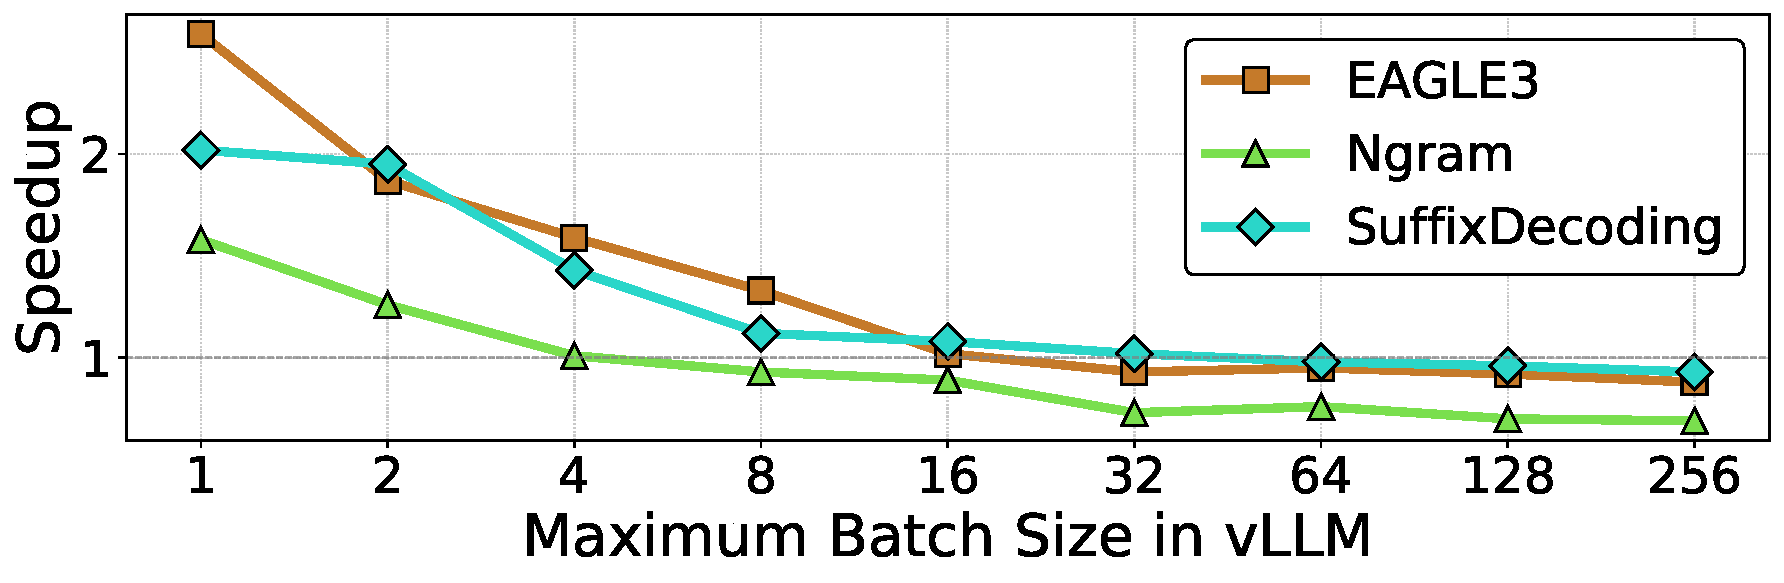
\includegraphics[width=0.48\textwidth]{Figures/moti_bz.pdf}
\caption{Speedup in terms of Goodput (number of generated tokens divided by the execution time)~\citep{liu2024optimizing} under various maximum batch size in vLLM for different speculative decoding algorithms on USACO dataset with Code Generation Agent implemented by Reflexion agentic workflow on Qwen-3-8B. }
\label{fig:moti_bz}
\end{figure}

To understand the cause of this degradation, we model the per-step execution time saving $\Delta T(b)$ of speculative decoding with batch size $b$ as:
\begin{align*}
\Delta T(b) &= T_{\text{base}}(b) - T_{\text{spec}}(b) \\
&\approx D(b)(1-\rho(b))t_A - D(b)\big(t_D(b) + t_V(b)\big) \\
&= D(b)\left[(1-\rho(b))t_A - t_D(b) - t_V(b)\right] \\
&\approx D(b)\left[(1-\rho(b))t_A - t_V(b)\right]
\end{align*}
where $D(b)$ denotes the number of drafted tokens in the current step, $\rho(b)$ is the rejection rate that is defined as the ratio of rejected tokens to proposed tokens for each request in the batch, $t_A$ is the per-token time saved by accepting a draft token, and $t_D(b)$ and $t_V(b)$ are the per-token draft and verification costs.

Since $t_D(b)$ is small and can be ignored, this formulation highlights two key factors that impact the efficiency: the rejection rate $\rho(b)$ and $D(b)\big(t_A - t_V(b)\big)$, which we call the utilization of the draft token budget. In general lower rejection rates and higher budget utilization bring in an ideal speculative decoding with larger speedups.


\subsection{Bottleneck Analysis} Motivated by the analysis above, we next examine how existing methods behave with respect to the rejection rate and the token budget utilization.

\noindent\textbf{Bottleneck of High Rejection Rate.} We record the rejection rate, defined as the ratio of rejected tokens to proposed tokens for each request in the batch from vLLM logs during Code Generation Agent inference. ~\cref{tab:rejection_rate} records the average rejection rate for different speculative decoding algorithms. As shown, existing speculative decoding methods suffer from extremely high rejection rates: EAGLE-3 exceeds 50\%, while NGram exceeds 85\% across most batch sizes. Such high rejection rates substantially limit the effective utilization of the draft token budget, directly contributing to the observed degradation in throughput speedup under large-batch settings for LLM agent inference.

\rejTable

\noindent\textbf{Bottleneck of Token Budget Under-Utilization.} We define the available token budget under batch size $b$ as $M(b) = AI - b$, where $AI$ denotes the arithmetic intensity of the deployed hardware for the LLM agent. This definition reflects the fact that, as the batch size increases, LLM inference—particularly the FFN layers—quickly becomes compute-bound and dominates end-to-end latency. As a result, the verification cost $t_V(b)$ increases and eventually approaches the per-token acceptance saving $t_A$, making the total execution time saving $\Delta T(b)$ become:
\begin{align*}
\Delta T(b)
&\approx D(b)\left[(1-\rho(b)) t_A - t_V(b)\right] \\
&= D(b)\left[(1-\rho(b)) t_A - t_A\right] = -D(b)\rho(b) t_A < 0
\end{align*}


\begin{figure}[t]
\centering
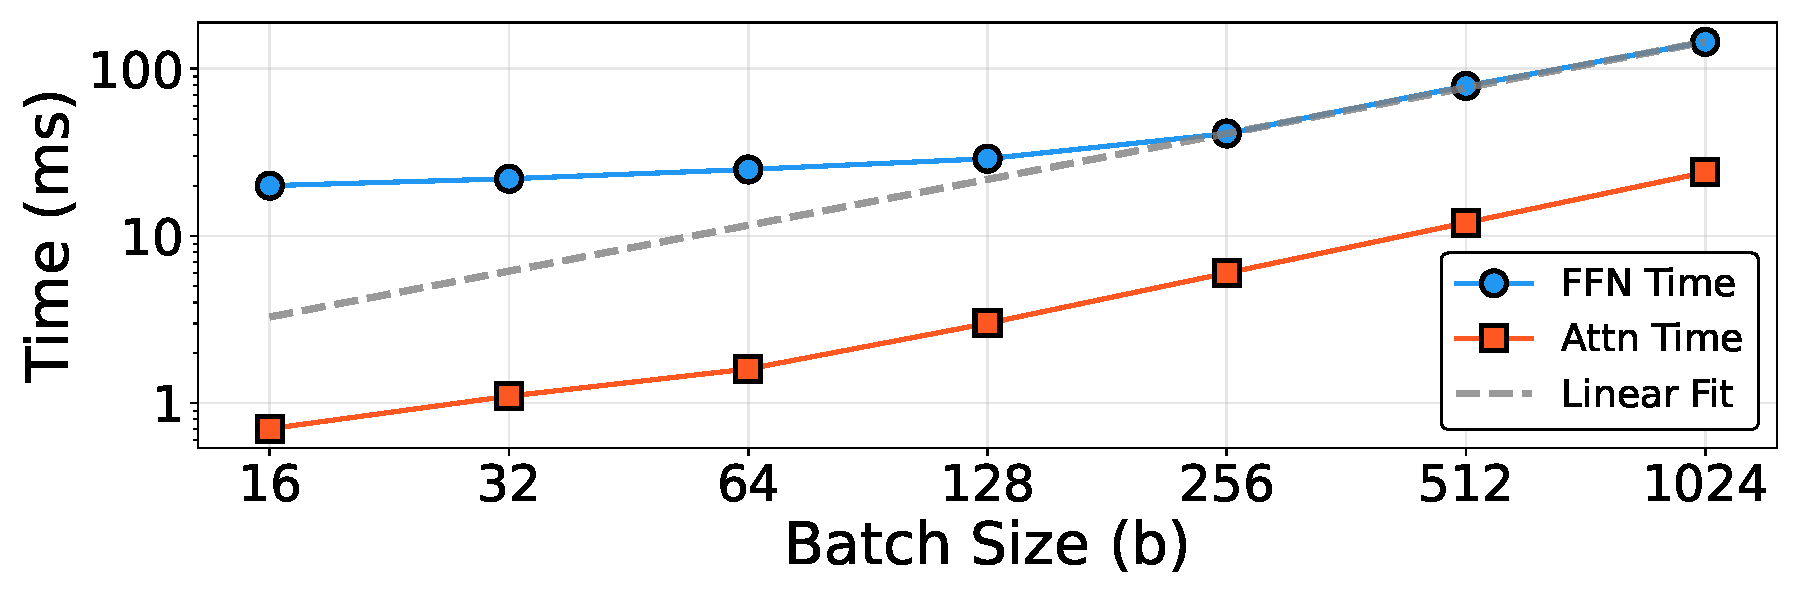
\includegraphics[width=0.48\textwidth]{Figures/moti_ffn_attn.pdf}
\caption{Execution time comparison for FFN and Attention modules of Qwen-3-8B under various batch size. }
\label{fig:moti_ffn_attn}
\end{figure}
To further illustrate this effect, we measure the per-layer decoding time of the FFN and attention modules of Qwen-3-8B using vLLM with FlashAttention-2 on an A100 GPU. The results are shown in~\cref{fig:moti_ffn_attn}. When the batch size exceeds 256, which matches the arithmetic intensity of the A100, the FFN latency grows linearly with batch size and quickly dominates the total decoding time. In this regime, decoding becomes compute-bound by the FFN, and the per-token verification cost $t_V(b)$ approaches the per-token autoregressive decoding cost $t_A$. As a result, the time saved by accepting one draft token is almost entirely offset by the cost of verifying it, leaving speculative decoding with little or no performance gain. This observation justifies our definition of the available token budget $M(b)$, which captures the diminishing headroom for speculative tokens as batch size increases.

\begin{figure}[t]
\centering
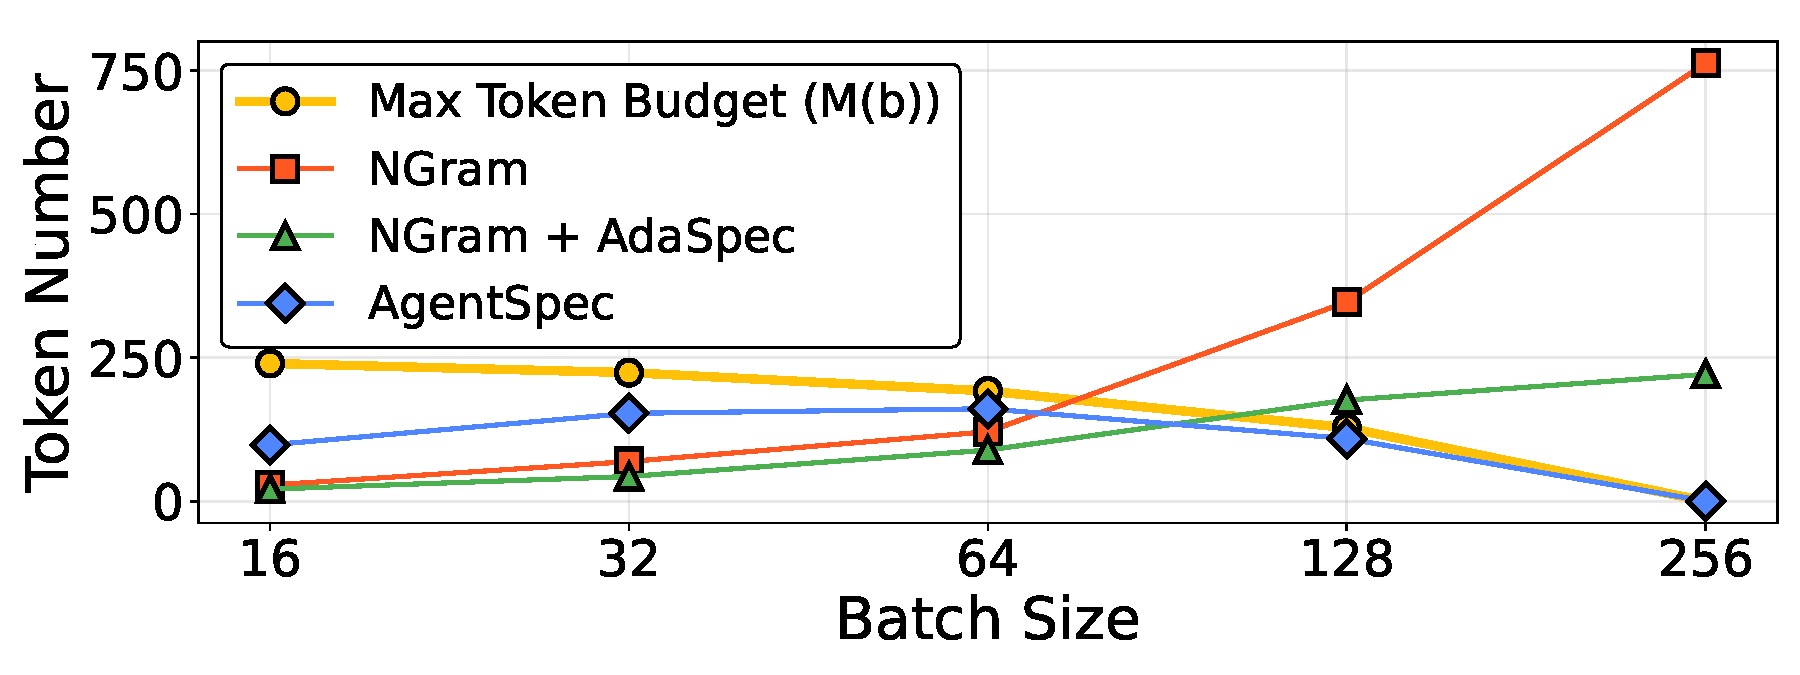
\includegraphics[width=0.48\textwidth]{Figures/moti_token_number.pdf}
\caption{Comparison between maximum token budget $M(b)$ and average proposed token number for batch inference of speculative decoding on Reflexion workflow.}
\label{fig:moti_token_number}
\end{figure}
We next record the total number of draft tokens generated per decoding step under different batch sizes and compare it with the available token budget $M(b)$. For a fair comparison, we also implement the budget allocation strategy from AdaSpec~\citep{10.1145/3772052.3772239}, which assigns draft tokens based on per-request acceptance rates. As shown in~\cref{fig:moti_token_number}, we have two key findings. (1) Existing speculative decoding methods severely under-utilize the available token budget, with the actual draft token count remaining far below or over $M(b)$ across all batch sizes.
(2) Existing allocation strategy fails to improve budget utilization, indicating that acceptance-rate–based budgeting is ineffective to improve the batch inference of speculative decoding for LLM agent.
% define max budget under various bz, budget vs draft tk ct
% solution: accept rate: 


\section{Method: AgentSpec}
\begin{figure}[ht]
\centering
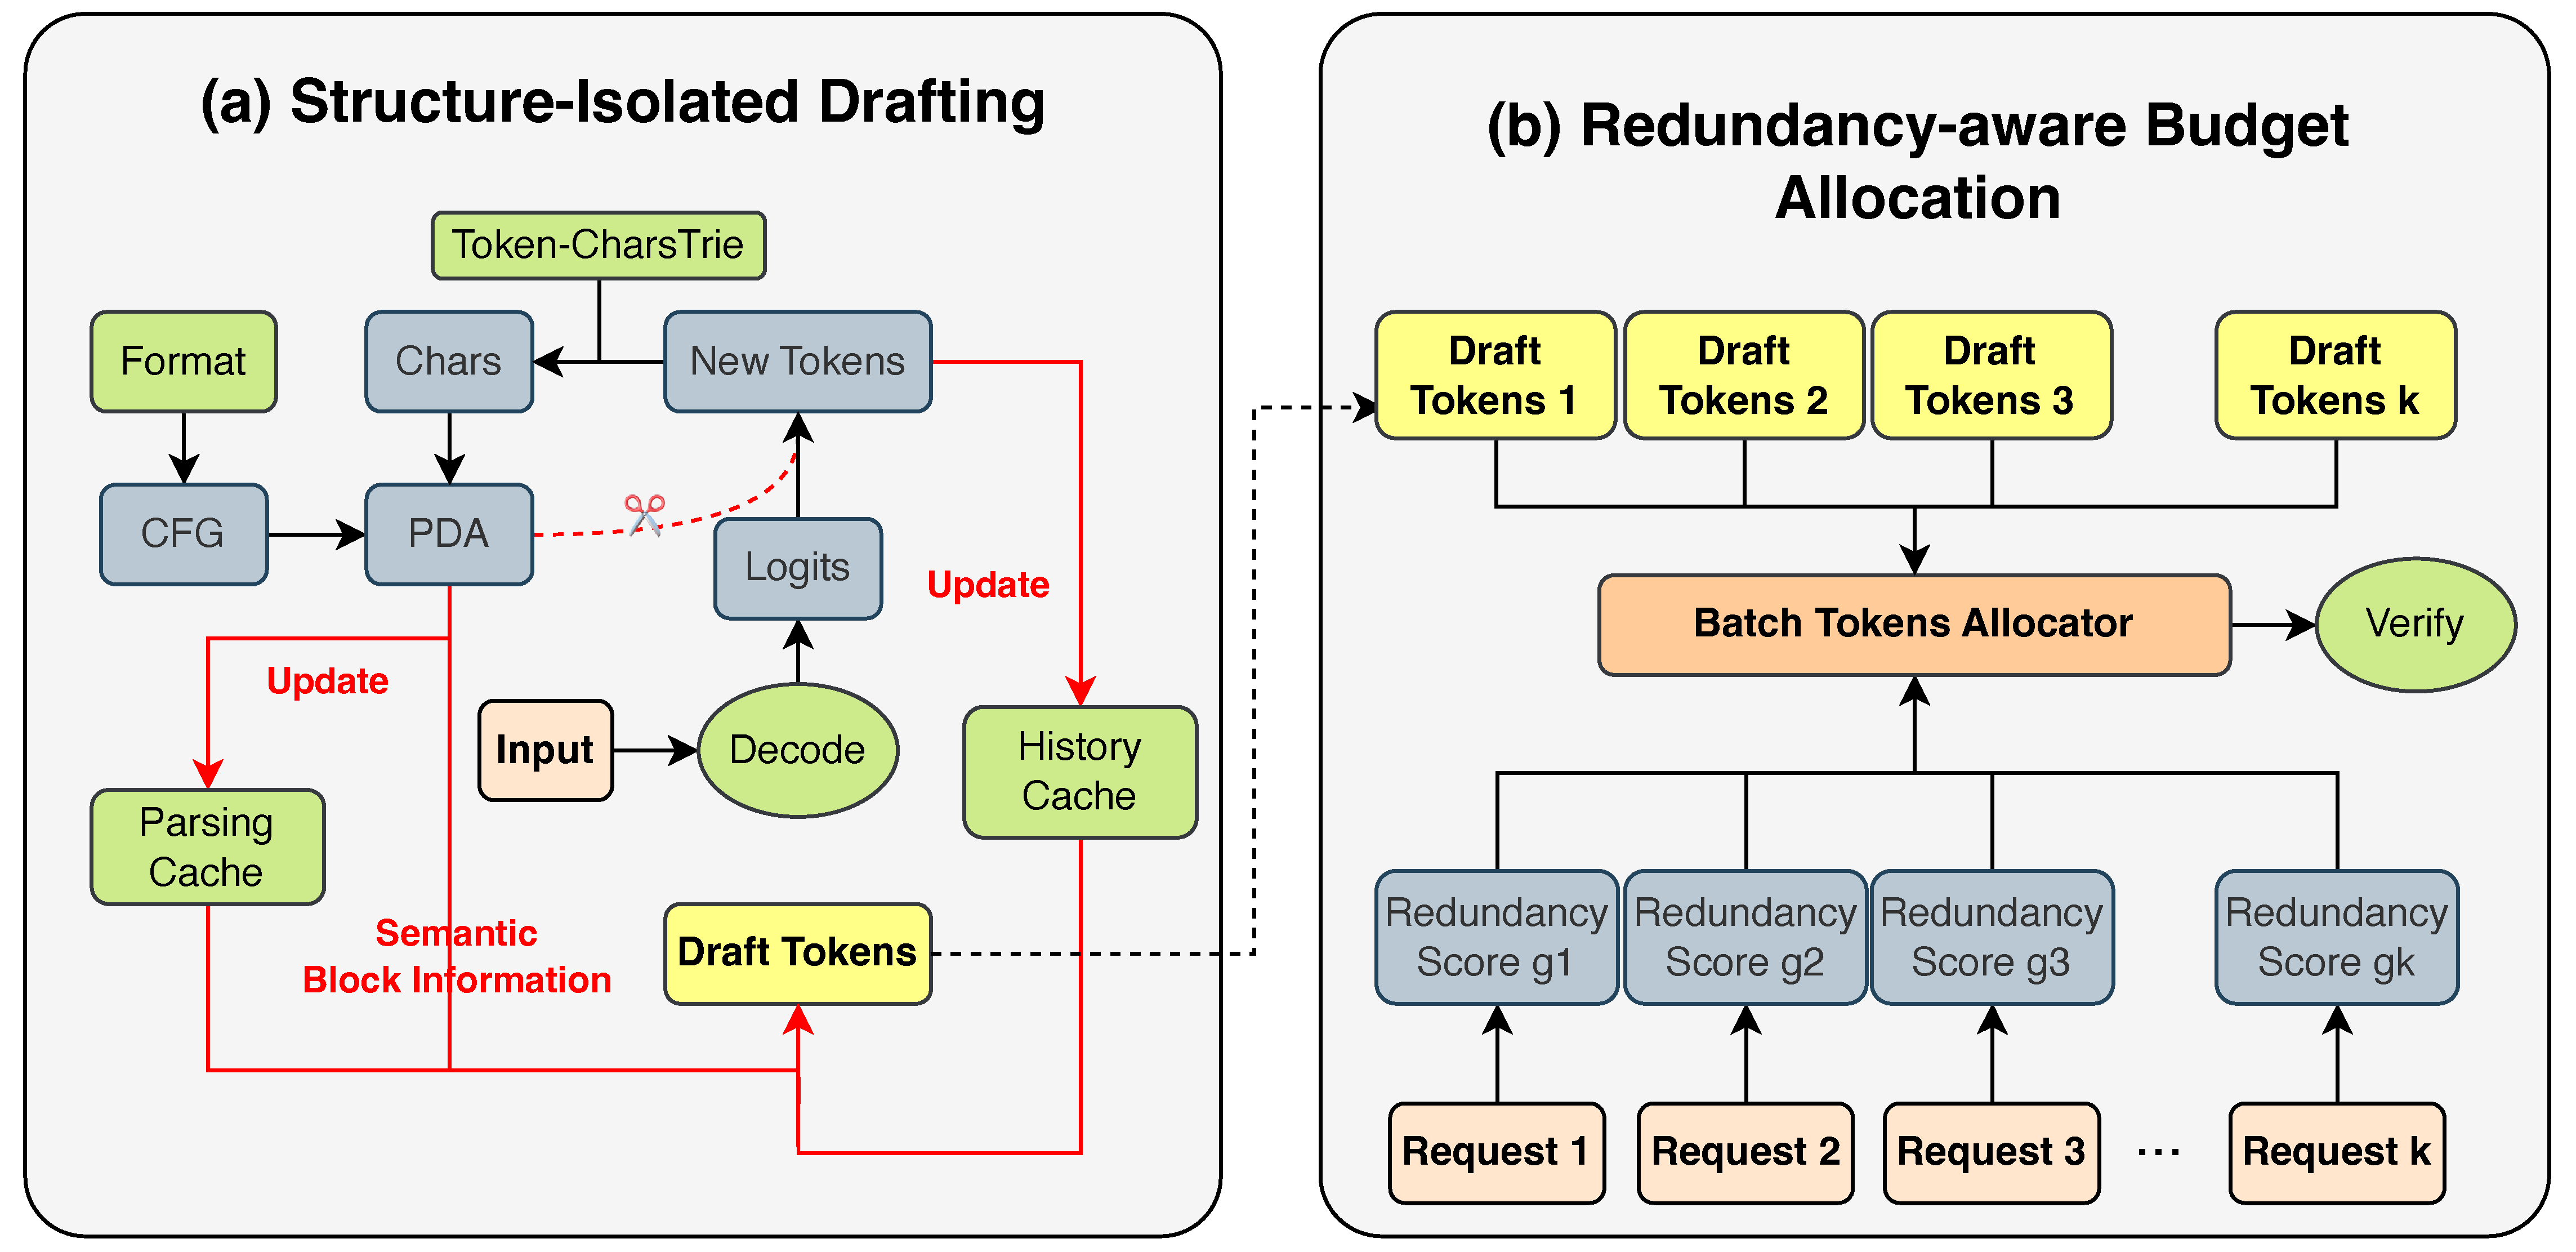
\includegraphics[width=0.48\textwidth]{Figures/AgentSpec.pdf}
\caption{Overview of \sysname.}
\label{fig:overview}
\end{figure}
\label{sec:method}
% \xin{Figure provides an overview of \sysname. }
The overview of \sysname is provided in~\cref{fig:overview}. At a high level, \sysname is a model-free speculative decoding algorithm designed for LLM agents. It requires the agent application to provide an agentic structure identifier alongside the input prompt to the LLM server, which enables the system to organize and retrieve historical context according to agent-specific execution structure.
%
During speculative drafting, \sysname retrieves draft candidates only from historical segments that belong to the same semantic group, thereby avoiding speculation across structurally mismatched contexts. Before verification, \sysname computes an integrated redundancy value for each request in the batch by combining local draft information with global generation history. It then allocates speculative token budgets across requests according to their relative redundancy scores and adjusts the draft length of each request accordingly.
%
In the following, we describe the two key components of \sysname—structure-isolated drafting and redundancy-aware budget allocation—in detail.


\subsection{Structure-Isolated Drafting}

\label{subsec:structured_isolated_drafting}
\noindent\textbf{Motivation:}
% 相同session的history matching数量 >> 不同session的history matching数量
% 相同session的相同sementic block内history matching的数量 >> 相同session的不同sementic block内history matching的数量
A key distinction between LLM agent applications and standard LLM workloads is that a single user query often spans multiple requests associated with different semantic blocks (e.g., reasoning, tool execution, and result interpretation). While generation patterns are highly consistent within the same semantic block, transitions across blocks or queries introduce substantial semantic shifts.

To quantify this effect, we analyze generation trajectories of Qwen-3-8B on the USACO dataset using a Reflexion-based code generation agent. For each request, we measure repeated token segments that reappear in previously generated content, distinguishing repetitions within the same block from those across different blocks or queries. A repetition is counted only if it contains at least $k$ consecutive tokens, with overlapping matches merged into their longest contiguous span. As shown in~\cref{fig:moti_repeated_ratio}, repeated token segments overwhelmingly occur within the same semantic block of a single query, whereas cross-block and cross-query repetitions are rare. This observation indicates that speculative drafting can be substantially improved by being aware of semantic block boundaries and query scope, thereby reducing unnecessary drafting and speculative rejections. In contrast, existing methods such as NGram and SuffixDecoding retrieve draft candidates from global generation history without such distinctions, leading to high rejection rates and wasted verification cost in agentic workloads.
\begin{figure}[t]
\centering
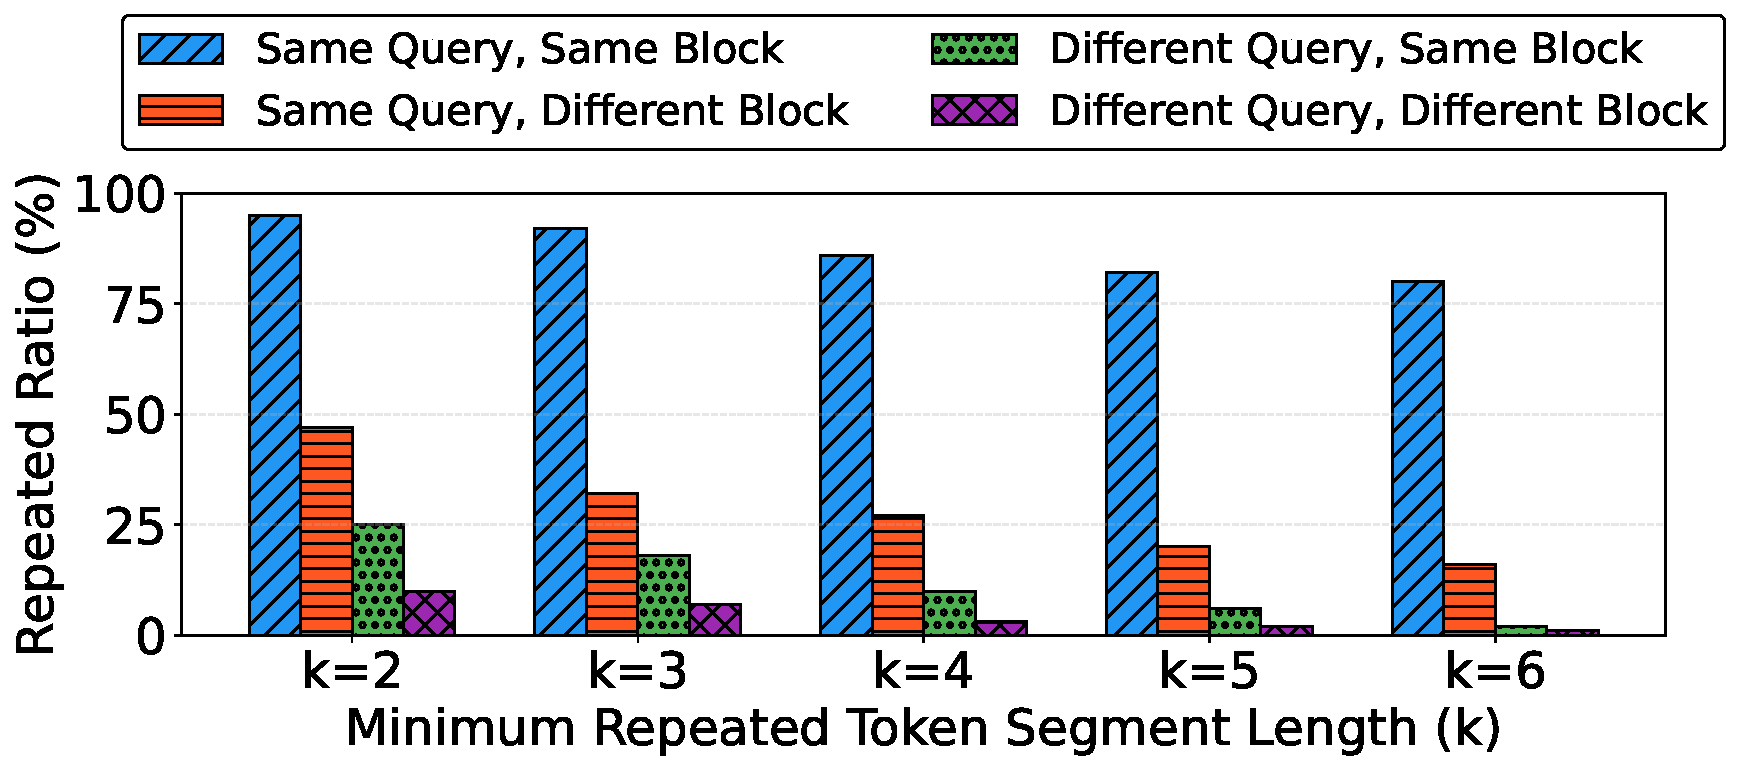
\includegraphics[width=0.48\textwidth]{Figures/moti_repeated_ratio.pdf}
\caption{Repeated token ratio under different minimum repeated span lengths $k$. The repeated ratio is defined as the total length of maximal repeated segments with at least $k$ consecutive tokens appearing in historical generations, normalized by the total generation length. Repetitions are categorized by whether they occur under the same or different user queries and within the same or different semantic blocks.}

\label{fig:moti_repeated_ratio}
\end{figure}

\noindent\textbf{Key Design:}
The pseudocode of structured-isolated draft of \sysname is provided in~\cref{algo:structure_isolated_drafting}. As shown, the algorithm requires the agent application to explicitly provide semantic structure identifier $S_i$ together with each generation request $r_i$ as below:
$$S_i=\{a_i, q_i, B_i\}$$
where $a_i$ denotes the agent application identifier, $q_i$ denotes the user query index that triggers the current request, and $b_i$ represents the list of $n$ semantic blocks $B_i = [b_i^1, b_i^2, b_i^3,...,b_i^n]$, defined by pairs of start and end string tags identified from previous generation history.

Mapping string-level semantic blocks to token-level generation is challenging due to subword tokenization, where token boundaries do not align with string boundaries. Direct token–string conversion during decoding is prohibitively expensive in common serving engines such as vLLM and sglang, where tokenization and decoding are handled by separate components.

To address this, \sysname adopts a design similar to XGrammar~\citep{DBLP:conf/mlsys/DongRCXZL025} by maintaining a cached token-to-string mapping $M$, enabling efficient online conversion of generated tokens without invoking the tokenizer. Based on this mapping, \sysname maintains a lightweight string-based pushdown automaton (PDA) $P$ on the server, which is incrementally updated to track the current semantic block.

For each request $r_i$, newly generated tokens are converted using $M$ and fed into the corresponding PDA $P(a_i, q_i)$ to identify the active semantic block $b_i^k$. \sysname maintains a separate structure-isolated cache for each semantic block and retrieves speculative drafts exclusively from the matched block, avoiding semantically irrelevant contexts and substantially reducing speculative rejections. As shown in~\cref{tab:rejection_rate}, \sysname achieves a rejection rate as low as 26\%, over 2$\times$ lower than existing baselines.


\subsection{Redundancy-aware Budget Allocation}
\label{subsec:redundancy_aware_budget_allocation}
\noindent\textbf{Motivation:} The pseudocode of the redundancy-aware budget allocation is shown in~\cref{algo:redundancy_aware_budget}.
To efficiently utilize the dynamic token budget in speculative decoding, more draft tokens should be assigned to requests with higher acceptance potential. Over-allocating tokens to low-acceptance requests wastes verification cost, while overly conservative allocation under-utilizes the available budget. The key challenge is thus to identify a reliable request-level signal that predicts draft acceptance.
%
In agent workloads, requests exhibit varying degrees of redundancy in their generation history. Intuitively, drafts aligned with repeated historical patterns are more likely to be accepted. To validate this intuition, we analyze generation traces from Qwen-3-8B on Code Generation Agent and measure draft redundancy as the fraction of matched historical continuations that fully accept the draft. As shown in~\cref{fig:redundancy_accept_map}, higher redundancy strongly correlates with higher acceptance rates, with the correlation strengthening as more matched continuations are observed.

\begin{figure}[t]
\centering
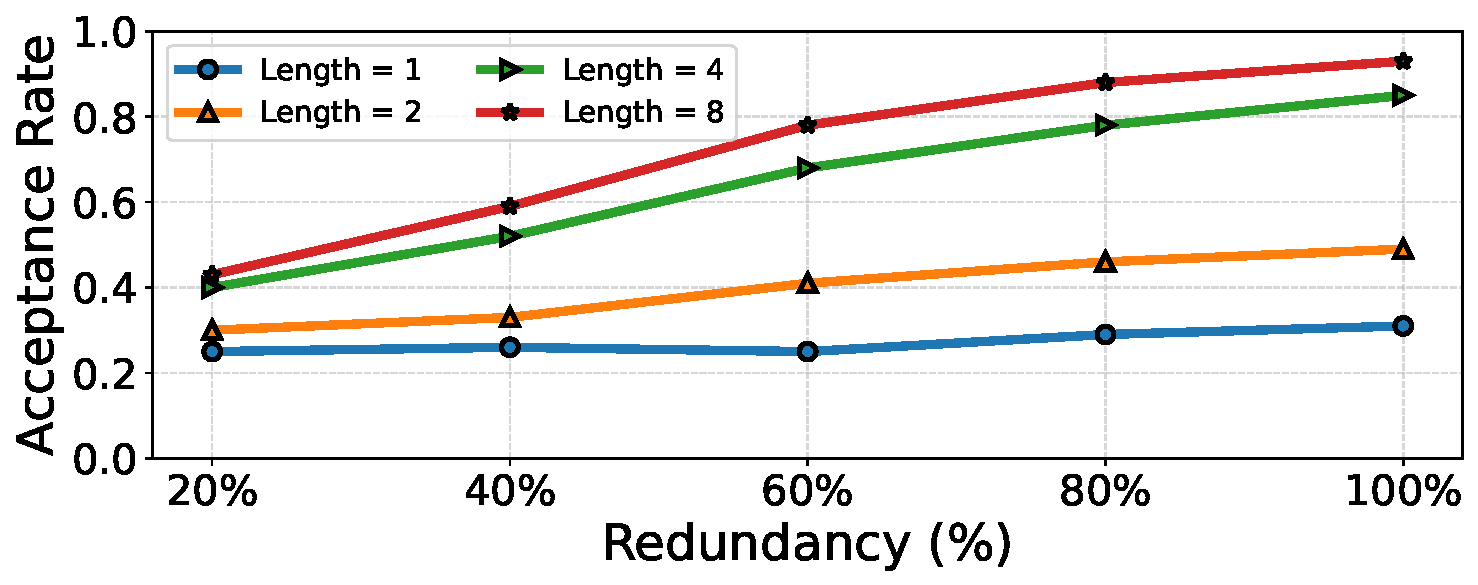
\includegraphics[width=0.48\textwidth]{Figures/redundancy_accept.pdf}
\caption{Acceptance ratio ($1-\rho(b)$ under different redundancy ratio with different matching pattern length.}
\label{fig:redundancy_accept_map}
\end{figure}

% 相同agent应用的接受率相近， 不同的差异明显
% 越一致，接受率越高 more consensus, more probable to accept
% model free的方法都是用continuation来做的

\noindent\textbf{Key Design:} 
% To estimate the acceptance likelihood of a speculative draft for each request in a batch, \sysname introduces a redundancy score $g$, defined as:
% \begin{equation}
% g(c, n)=\frac{c}{n} \cdot p(n)=\frac{c}{n} \cdot\left[g_{\min }+\left(1-g_{\min }\right)\left(1-e^{1-n}\right)\right]
% \end{equation}
% where $n$ denotes the number of candidate continuations found in the generation history under the same semantic block and the same user query, and $c$ denotes the number of continuations that agree on the most frequent continuation prefix. The hyperparameter $g_{min}$ controls the minimum confidence when historical evidence is scarce.
%
% The ratio $\frac{c}{n}$ captures the consensus among candidate continuations: a larger value indicates higher redundancy and a higher likelihood that the proposed draft will be accepted. However, empirical results in the motivation part show that when $n$ is small, acceptance rates remain low even if $\frac{c}{n}$ is large. To account for this effect, we introduce the exponential saturation term $p(n)$, which downweights redundancy estimates under low-support scenarios.
%
% Given the redundancy scores, \sysname computes the total speculative token budget as
% \begin{equation}
% B_t=\left\lfloor\frac{\alpha}{b z}\right\rfloor
% \end{equation}
% where $bz$ is the current batch size and $\alpha$ is a tunable hyperparameter that controls the overall speculative budget. For each request $r_i$ in the batch, \sysname retrieves all $n_i$ candidate draft paths from the history that belong to the same semantic block and user query. A lightweight n-gram index is then constructed to identify the most frequent continuation prefix $CT_i$ and compute its redundancy score $g_i$. After obtaining ${(CT_i, g_i)}$ for all requests, \sysname allocates a per-request draft length
% \begin{equation}
% L_i=\max \left(\left|C T_i\right|, B_t \cdot \frac{g_i}{\sum_j g_j}\right)
% \end{equation}
% prioritizing requests with higher redundancy while ensuring that each request can draft at least its most confident continuation prefix. As shown in~\cref{fig:moti_token_number}, \sysname consistently ensures a batch draft token number lower than the maximum budget $M(b)$, and generally approaches it with the increase of batch size, indicating a good utilization of the available token budget during agent batch inference.
To estimate the acceptance likelihood of a speculative draft for each request,
\sysname introduces a redundancy score $g$:
\begin{equation}
g(c,n) = \frac{c}{n}\cdot p(n), \;
p(n) = g_{\min} + (1-g_{\min})(1-e^{1-n}),
\end{equation}
where $n$ is the number of candidate continuations retrieved from the generation
history under the same semantic block and user query, and $c$ is the number of
continuations agreeing on the most frequent prefix. The ratio $c/n$ captures the
consensus among candidates, while the saturation term $p(n)$ downweights unreliable
estimates when historical support is limited. The hyperparameter $g_{\min}$ controls
the minimum confidence under low-support scenarios.

Given the redundancy scores, \sysname computes the batch-level speculative token
budget as
\begin{equation}
B_t = \left\lfloor \frac{\alpha}{bz} \right\rfloor,
\end{equation}
where $bz$ is the batch size and $\alpha$ controls the overall speculative budget.
For each request $r_i$, \sysname retrieves candidate drafts within the same semantic
block and query, identifies the most frequent continuation prefix $CT_i$, and
computes its redundancy score $g_i$. The per-request draft length is then allocated as
\begin{equation}
L_i = \max\!\left(|CT_i|,\; B_t \cdot \frac{g_i}{\sum_j g_j}\right),
\end{equation}
prioritizing requests with higher redundancy while ensuring that each request can
draft at least its most confident prefix.

As shown in~\cref{fig:moti_token_number}, \sysname consistently keeps the total number
of drafted tokens below the maximum budget $M(b)$ and approaches it as batch size
increases, indicating effective utilization of the available speculative budget.


\section{Experiments}
\label{sec:experiments}
\eeTable

\begin{figure*}[t]
\centering
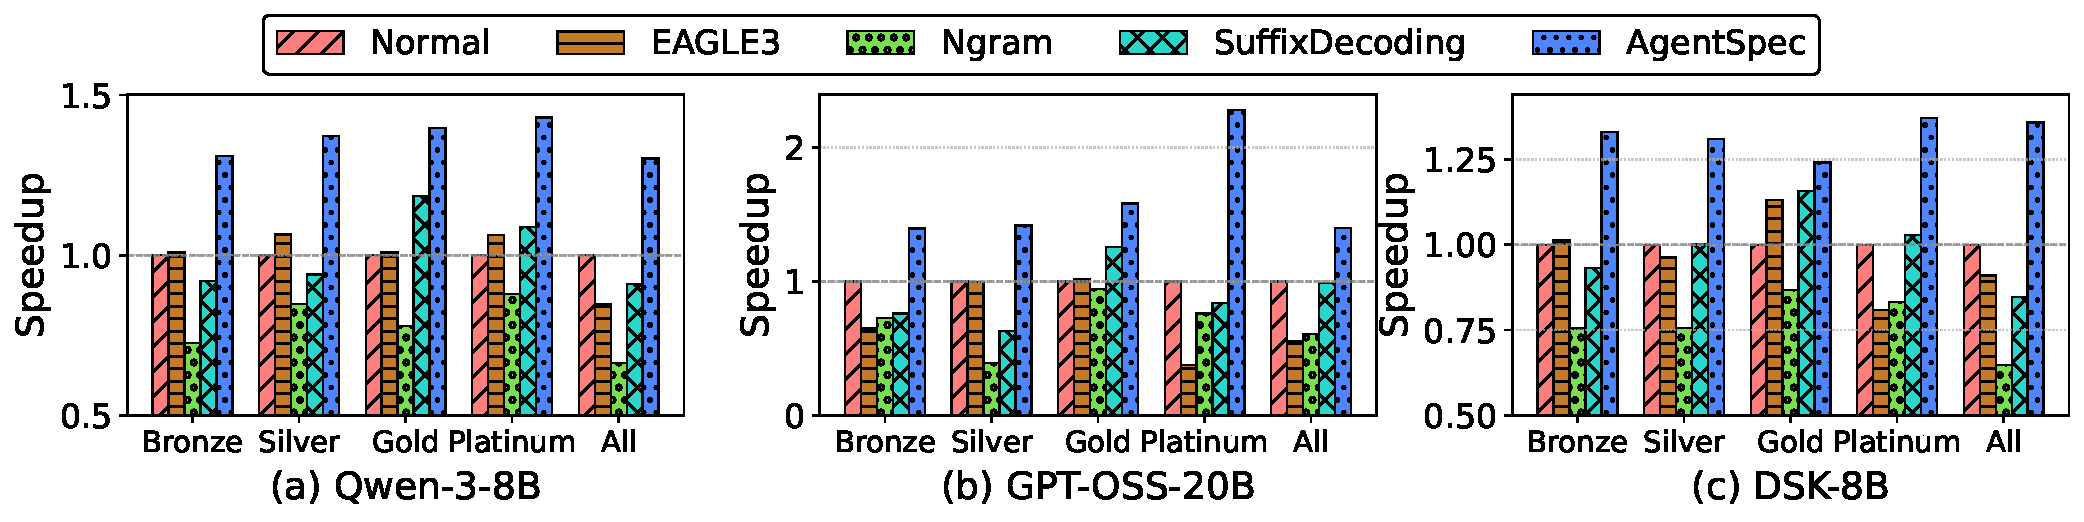
\includegraphics[width=0.98\textwidth]{Figures/e2e_throughput.pdf}
\vspace{-3mm}
\caption{Speedup in terms of Goodput (token/s) for \sysname and baselines compared with normal autoregressive decoding on all subsets in USACO dataset with Code Generation Agent implemented by Reflexion agentic workflow on three different models.}
\vspace{-3mm}
\label{fig:e2e_subset}
\end{figure*}

\subsection{Experimental Setups}
\label{subsec:setup}

\noindent\textbf{Baselines.} We compare \sysname against two groups of methods: (1) Draft-model-based speculative decoding methods: EAGLE-3~\citep{DBLP:journals/corr/abs-2503-01840} and MTP~\citep{DBLP:journals/corr/abs-2505-07608}. (2) Draft-model-free speculative decoding methods: NGram~\citep{saxena2023prompt} and SuffixDecoding~\citep{oliaro2025suffixdecoding}. All baselines are evaluated under identical serving configurations to ensure a fair comparison.

\noindent\textbf{Models and Datasets.} 
To demonstrate the generality of \sysname, we evaluate its performance on four models from different families, including Qwen-3-8B~\citep{DBLP:journals/corr/abs-2505-09388}, GPT-OSS-20B~\citep{DBLP:journals/corr/abs-2508-10925}, Deepseek-R1-Distill-Llama-8B~\citep{DBLP:journals/corr/abs-2501-12948}, and MiMo-7B~\citep{DBLP:journals/corr/abs-2505-07608}.
%
We evaluate on four most popular agentic workloads covering two main types. The first is workflow-based agent workload, including Code Generation that is implemented with Reflexion framework~\citep{DBLP:conf/nips/ShinnCGNY23} and tested on USACO benchmark~\citep{DBLP:journals/corr/abs-2404-10952} with multiple difficulty subsets (Bronze, Silver, Gold, and Platinum), and Deep Research that is implemented with LangChain DeepResearch framework~\citep{langchain2026dr} and tested on DeepResearch-Bench benchmark~\citep{DBLP:journals/corr/abs-2506-11763} with three different levels of tasks that require long-horizon reasoning and document synthesis. 
%
The second is model-based agentic workloads, including SWE-Bench-Lite~\citep{DBLP:conf/iclr/JimenezYWYPPN24} and GAIA~\citep{DBLP:conf/iclr/MialonF0LS24} on OpenHands platform~\citep{DBLP:conf/iclr/0001LSXTZPSLSTL25}.
%
Finally, we evaluate \sysname on Spec-Bench~\citep{DBLP:conf/acl/XiaYDW00L0S24} to test its performance enhancement on non-agentic data.

\noindent\textbf{Metrics.} Following the standards of Turbospec~\citep{liu2024optimizing}, we use goodput, defined as the total number of generated tokens divided by the execution time of the entire agent workload, as the main metric to evaluate the goodput of \sysname and its baseline methods. We also report speedup in terms of goodput for a clearer comparison, as well as latency~\citep{DBLP:journals/corr/abs-2502-13965}, which is defined as the end-to-end execution time from when a user query enters the agent environment to when the final response is returned.

\noindent\textbf{Implementation Details.} To ensure a fair and realistic comparison, we implemented \sysname and evaluate its performance with baseline methods in vLLM~\citep{DBLP:conf/sosp/KwonLZ0ZY0ZS23}, a production-style LLM serving engine. All other baseline methods are also evaluated with the official implementation provided in vLLM under maximum batch size 256. The detailed configurations in vLLM for running the evaluation is provided in~\cref{appendix:vllm_configration_details}. 

\subsection{End-to-End Comparison}
\label{subsec:end_to_end_comparison}
We first compare the end-to-end efficiency of \sysname against existing baseline methods on two agent applications—Deep Research Agent and Code Generation Agent—as well as two agent benchmarks, GAIA and SWE-Bench, across three different LLMs: Qwen-3-8B, GPT-OSS-20B, and DeepSeek-Distill-LLaMA-8B.
The results are shown in~\cref{tab:e2e_comparison}. \sysname consistently outperforms all baseline speculative decoding methods in terms of efficiency, achieving up to $104\%$ higher goodput. Notably, the goodput of most baseline methods is even lower than that of standard autoregressive decoding, indicating limited benefits in agent workloads.
In contrast, \sysname consistently delivers improved goodput across all agent workloads and model settings, attaining up to a 2.02$\times$ speedup over autoregressive decoding.

\subsection{Comparison with Different Execution Patterns} Even within the same agent workload, problem difficulty can lead to distinct agent execution patterns. A common phenomenon is that more challenging problems induce longer contexts and a larger number of generation steps, as the agent needs to issue more LLM requests to complete the task. To demonstrate the generality of \sysname, we evaluate its efficiency using the Code Generation Agent across all subsets of the USACO dataset, with difficulty levels ranging from Bronze to Platinum. As shown in~\cref{fig:e2e_subset}, \sysname consistently achieves better speedup than other speculative decoding methods across all difficulty subsets and LLMs. More importantly, \sysname also consistently outperforms standard autoregressive decoding, achieving up to a 2.2$\times$ speedup on the USACO subsets.

\subsection{Comparison on Non-Agentic Benchmark}
\label{subsec:spec_bench}
Following the experimental protocol of~\citep{oliaro2025suffixdecoding}, we conduct the evaluation on a non-agentic benchmark Spec-Bench~\citep{DBLP:conf/acl/XiaYDW00L0S24} using Qwen-3-8B. Unlike agentic workloads, which often involve multi-turn requests for a single query and contain explicit semantic structures, Spec-Bench contains fewer repeated historical generations, making it more challenging to utilize history information for drafting. However, as shown in~\cref{tab:qwen_specbench}, \sysname still consistently achieves higher efficiency than both speculative decoding baselines and standard autoregressive decoding across all subsets as well as the full Spec-Bench benchmark. 

\mimoTable

\specbenchTable

\subsection{Comparison with Multi-Token Prediction}
\label{subsec:mtp_comparison}
Multi-Token Prediction (MTP) is a recent speculative decoding paradigm that jointly trains an MTP module as the draft model during the pre-training stage of the target model. To further demonstrate the effectiveness of \sysname, we compare its efficiency with MTP speculative decoding method using MiMo-7B on the Code Generation Agent over the USACO dataset. As shown in~\cref{tab:mimo_usaco}, MTP exhibits limited efficiency gains under batched LLM agent inference. In contrast, \sysname consistently achieves higher efficiency than MTP and maintains a clear speedup over standard autoregressive decoding on MiMo-7B.

\begin{figure}[t]
\centering
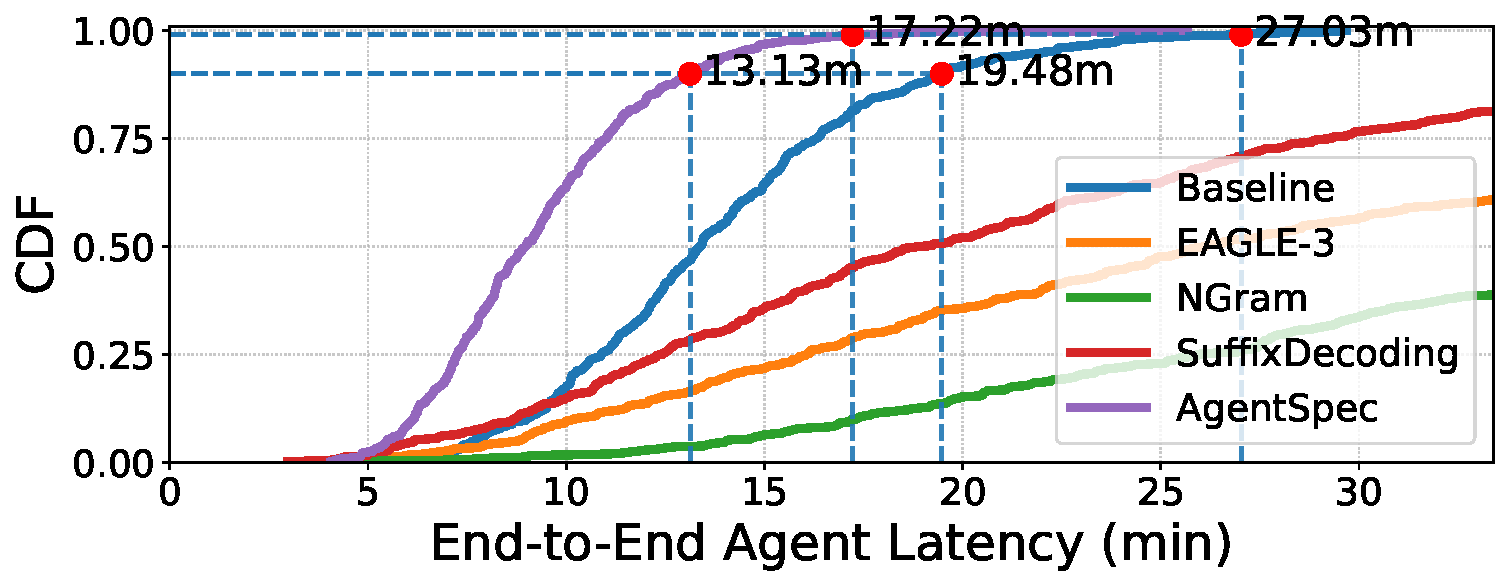
\includegraphics[width=0.48\textwidth]{Figures/e2e_latency.pdf}
\caption{Tailed latency analysis for \sysname and baselines on Code Gen agentic workflow.}
% \vspace{-3mm}
\label{fig:e2e_latency}
\end{figure}

% \begin{figure}[t]
% \centering
% \includegraphics[width=0.48\textwidth]{Figures/verification_cost.pdf}
% \caption{Drafting time cost for \sysname and baselines under different batch size.}
% % \vspace{-8mm}
% \label{fig:verification_cost}
% \end{figure}


\breakdownTable 

\subsection{Latency Analysis}
\label{subsec:tailed_latency_analysis} 
\noindent\textbf{Tailed Latency.} We further analyze the end-to-end program latency, defined as the time elapsed from when a user query is submitted to the agent application to when the final output is returned. The CDF of the tail latency is shown in~\cref{fig:e2e_latency}.
\sysname consistently achieves lower latency than baseline speculative decoding methods, and reduces tail latency by up to 1.47$\times$ and 1.39$\times$ compared to standard autoregressive decoding at the P90 and P99 percentiles, respectively.

\noindent\textbf{Execution Breakdown Analysis.}  We have performed fine-grained analysis including both drafting and verification costs on Reflexion Agentic Workflow. The results in~\cref{tab:runtime_breakdown} show that \sysname significantly reduces verification overhead compared to baselines, which is the dominant factor in overall speedup.  \sysname incurs slightly higher drafting overhead than NGram and SuffixDecoding. This additional cost mainly stems from maintaining the PDA in the structure-isolated drafting component and computing redundancy statistics in the redundancy-aware budget allocation module.
Nevertheless, the overhead remains negligible, amounting to less than 2 ms, and the overall drafting cost of \sysname is still lower than all baseline methods.


\subsection{Ablation Studies}
\label{subsec:ablation_study}
%
\sensitivityTable
% \acclenTable

\textbf{Modular Sensitivity Study.} We evaluate the separate contributions of the two key components (i.e., structure-isolated drafting and redundancy-aware budget allocation) of \sysname. 
%
Let \sysname \texttt{(S)} denote the version of \sysname with structure-isolated drafting only; \sysname \texttt{(R)} denote the version of \sysname with SuffixDecoding and redundancy-aware budget allocation.
%; and \sysname  denote the version of \sysname with both truncation-aware data whitening and parameter update with sequential low-rank approximation.
As shown in~\cref{tab:sensitivity}, we have three observations. 
%
(1) \sysname\texttt{(S)}, \sysname\texttt{(R)} and \sysname consistently outperform existing speculative decoding methods. 
%
(2) \sysname consistently outperforms both \sysname\texttt{(S)} and \sysname\texttt{(R)}.
%
This result demonstrates the unique contribution from each of the two key components and the importance of combining both components to achieve the best performance.
%
(3) Comparing between \sysname\texttt{(S)} and \sysname\texttt{(R)}, \sysname\texttt{(S)} achieves a higher speedup compared to \sysname\texttt{(R)}, indicating that structure-isolated drafting plays a more significant role than redundancy-aware budget allocation.

\noindent\textbf{Performance without Explicit Semantic Structures.} Since the structure-isolated drafting component of \sysname requires the agent application to provide explicit semantic block boundaries, some real-world agentic workloads may not expose such structure during generation. To assess the generality of \sysname, we have evaluated a variant that operates without semantic structure inputs, denoted as \sysname\texttt{(N)}. As shown in~\cref{tab:sensitivity}, \sysname\texttt{(N)} consistently outperforms both speculative decoding baselines and standard autoregressive decoding.
%Moreover,  We have instrumented vLLM to record the acceptance length at each verification step on the CodeGen agentic workload, and analyzed its distribution. We observe that while repetitive agentic template tokens exhibit slightly higher acceptance lengths than other tokens, they account for only a small portion of the overall generated tokens (8\% for Qwen-3-8B with thinking enabled). As a result, the average acceptance length over the full sequence remains close to that of non-template tokens. This indicates that the performance gains are not dominated by a small subset of repetitive agentic template tokens, but instead arise from consistent improvements across the majority of decoding steps.

\noindent\textbf{Performance Under Various Maximum Batch Size.} We next evaluate the performance of \sysname under different maximum batch size configurations in the vLLM engine. As shown in~\cref{fig:ablation}(a), while some existing speculative decoding methods (e.g., SuffixDecoding) achieve higher efficiency than standard autoregressive decoding at small batch sizes, their speedup gradually degrades and can even fall below autoregressive decoding as the maximum batch size increases.
In contrast, \sysname consistently maintains superior efficiency across all batch size configurations, outperforming both speculative decoding baselines and standard autoregressive decoding.

\begin{figure}[t]
\centering
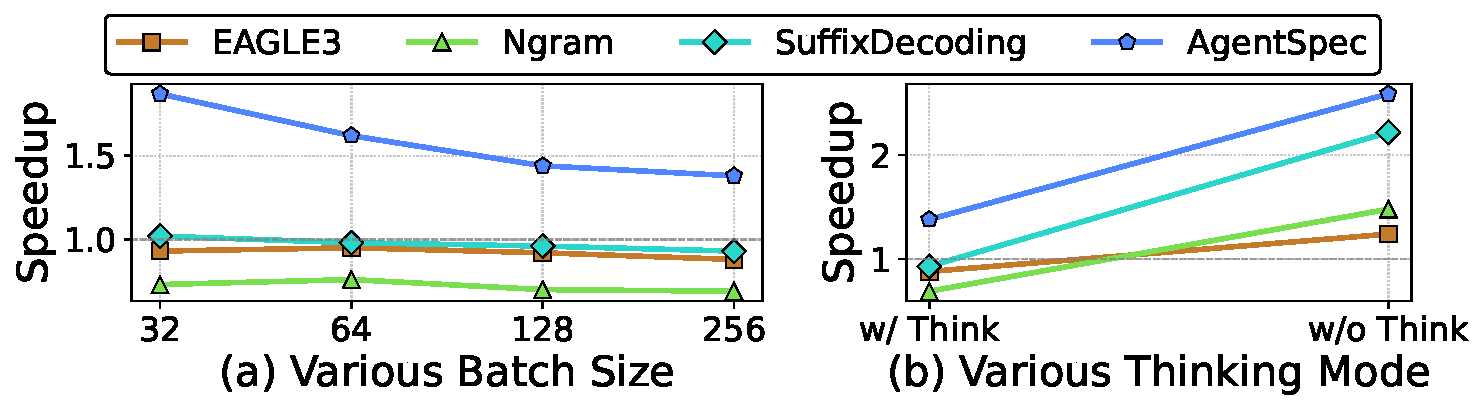
\includegraphics[width=\linewidth]{Figures/e2e_ablation.pdf}
\caption{Speedup in terms of Goodput (tokens/sec) of \sysname and baselines on workload of code generation agent under various maximum batch size and different thinking modes.}
\label{fig:ablation}
\end{figure}


\noindent\textbf{Performance in Different Thinking Modes.} Recent reasoning-oriented LLMs allow users to adjust thinking modes, which can substantially affect both the generated content and output length in agent applications.
To study this effect, we evaluate \sysname on Qwen-3-8B under two thinking modes: w/ think and w/o think~\citep{DBLP:journals/corr/abs-2505-09388}.
As shown in~\cref{fig:ablation}(b), \sysname consistently achieves superior performance across both modes. Notably, under the w/o think setting, \sysname is over 2.5$\times$ faster than standard autoregressive decoding.

\section{Conclusion}
\label{sec:conclusion}

% In this paper, we presented \sysname, a SVD-based
% LLM compression method. 
% %
% \sysname proposes a novel truncation-aware data whitening strategy to guide which singular values to be truncated with minimal compression loss. It also introduces a layer-wise closed-form model parameter update scheme to compensate for accuracy degradation under high compression ratios.
% %
% We have demonstrated the effectiveness of \sysname on 11 datasets and seven models from three LLM families at four scales and have shown its superiority over state-of-the-arts. We also show its effectiveness in further enhancing the performance of other LLM compression methods as well as KV cache reduction. 
%consistently outperforms state-of-the-art SVD-based LLM compression methods. Moreover, we demonstrated its performance on integrating with other compression techniques and on reducing runtime memory by reducing KV cache size.
In this paper, we presented \sysname, a speculative decoding algorithm tailored for batch inference of LLM agents.
%
\sysname introduces structure-isolated drafting to constrain speculation to semantically coherent segments of the agent workflow, achieving extremely low rejection rates. It also proposes redundancy-aware budget allocation to better exploit dynamically available token budgets using agent-level redundancy.
%
% We implement and evaluate \sysname in vLLM.
Our experimental results demonstrate the superiority of \sysname over state-of-the-art baselines.
%
% We systematically analyzed why existing speculative decoding methods fail to scale to large batch sizes, and identified high rejection rates and token budget under-utilization as the two dominant bottlenecks.
%
% Extensive experiments on realistic code-generation agent workloads demonstrate that \sysname consistently outperforms state-of-the-art speculative decoding methods across a wide range of batch sizes, recovering stable and substantial throughput gains where existing methods collapse.

\section*{Limitation} AgentSpec introduces a lightweight interface between the agent and serving system, which may require minor adaptation in practice. In addition, its structure-isolated drafting component benefits from explicit semantic block information. Although AgentSpec can operate without such metadata, its speedup may depend on the amount of repeated generation patterns available in the workload.

\section*{Ethical Considerations}
AgentSpec is a serving-time acceleration method for LLM-based agents. It does not modify model parameters, training data, or the generation objective, and therefore is not intended to change the output distribution or content policy of the underlying model. Existing safety mechanisms for autoregressive decoding, such as content moderation, tool-use control, and deployment restrictions, should remain applicable when AgentSpec is enabled. Improving inference efficiency may reduce the cost of deploying LLM agents at scale, which can benefit practical applications but may also lower the barrier for misuse, such as automated spam generation or unsafe tool-use workflows. We therefore encourage responsible deployment with appropriate safeguards, including rate limiting, permission control, and monitoring. AgentSpec requires only lightweight semantic structure metadata from the agent application; such metadata should describe workflow structure rather than private or sensitive user information. Our experiments use publicly available benchmarks and do not require collecting additional private user data.

%\input{7_ack}




% \input{draft}
% \vspace{-2mm}
\setcitestyle{numbers}
% \bibliographystyle{unsrt} %unsrt
% \bibliographystyle{unsrtnat} %unsrt
\bibliography{Reference}

%%%%%%%%%%%%%%%%%%%%%%%%%%%%%%%%%%%%%%%%%%%%%%%%%%%%%%%%%%
%\newpage
%\section*{Checklist}
%\appendix
%\clearpage
%\input{8_supplementary}
\appendix
% %%%%%%%%%%%%%%%%%%%%%%%%%%%%%%%%%%%%%%%%%%%%%%%%%%%%%%%%%%%%%%%%%%%%%%%%%%%%%%%
% %%%%%%%%%%%%%%%%%%%%%%%%%%%%%%%%%%%%%%%%%%%%%%%%%%%%%%%%%%%%%%%%%%%%%%%%%%%%%%%
% % APPENDIX
% %%%%%%%%%%%%%%%%%%%%%%%%%%%%%%%%%%%%%%%%%%%%%%%%%%%%%%%%%%%%%%%%%%%%%%%%%%%%%%%
% %%%%%%%%%%%%%%%%%%%%%%%%%%%%%%%%%%%%%%%%%%%%%%%%%%%%%%%%%%%%%%%%%%%%%%%%%%%%%%%
\newpage
\appendix
\section{Appendix.}
\subsection{Experiment Configuration Details}
\label{appendix:vllm_configration_details}
We implement \sysname and conduct all experiments using the vLLM v0.12.0 V1 engine. For a fair comparison, we directly run the official implementations of all baseline methods with their default configurations provided by vLLM. We run each experiment on NVIDIA A100 80G GPUs with fix the maximum batch size and serving parameters for all methods. Unless otherwise specified, all goodput and speedup numbers are averaged over five times measurements controlled with various seed numbers and under the default maximum batch size 256 in vLLM.

Specifically, for NGram, we set \lstinline|num-speculative-tokens| to 5 and \lstinline|ngram-prompt-lookup-max| to 4; for SuffixDecoding, we set \lstinline|num-speculative-tokens = 32|.
% For EAGLE-3, we set the draft models as: Qwen-3-8B (\texttt{AngelSlim/Qwen3-8B\_eagle3}), GPT-OSS-20B (\texttt{RedHatAI/gpt-oss-20b-speculator.eagle3}), and DSK-Distill-8B (\texttt{yuhuili/EAGLE3-DeepSeek-R1-Distill-LLaMA-8B}), and \lstinline|num-speculative-tokens| to 2.

We use FlashAttention-2 as the attention backend and adopt the default maximum batch size in vLLM (256). For MTP, we directly use the official MTP module provided by MiMo-7B-RL during inference.

For \sysname, the speculation length dynamically adapts to the ongoing batch size and therefore does not require any speculation-length hyperparameters at launch time. Instead, \sysname requires the agent application to provide high-level contextual information, including the agent’s semantic structure and the query index of the current request.

Concretely, we extend the vLLM engine with three additional parameters—\lstinline|structure: string|, \lstinline|query-id: int|, and \lstinline|agent-id: int|—which can be passed by the agent application at inference time. The \lstinline|structure| field encodes the paired delimiters of semantic blocks (e.g., code blocks, tool calls, and mathematical expressions) used by \sysname for redundancy-aware speculation. An example API request is shown in Listing~\ref{lst:redundancy}.

\begin{lstlisting}[language=Python, caption={Example of API request command when using \sysname in vLLM}, label={lst:redundancy}]
resp = await client.chat.completions.create(
        model="Qwen/Qwen3-8B",
        messages=[
            {"role": "system", "content": "Respond in Korean."},
            {"role": "user", "content": f"Say hi. (req {i})"},
        ],
        temperature=0.6,
        extra_body={
        "query_id": 1,
        "agent_id": 1,
        # Code Structure and Math Structure
        "structure": "[
            [("```python", "```"), ("<tool_call>", "<\tool_call>")],
            [("\[", "\]"), ("\(", "\)"), ("$$", "$$"), ("$", "$")]
        ]",
    )
\end{lstlisting}


\begin{table}[ht]
    \centering
    % \begin{minipage}{.43\textwidth}
    %     \adaTable
    % \end{minipage}
    % \hspace{0.1cm}
    \begin{minipage}{.46\textwidth}
        \GPUTable
    \end{minipage}%
\end{table}

\subsection{Algorithm Pseudocode}
\cref{algo:structure_isolated_drafting} shows the pseudocode of the first component of \sysname, Structure-Isolated Drafting. \cref{algo:redundancy_aware_budget} shows the pseudocode of the second component of \sysname, Redundancy-Aware Budget Allocation.
\begin{algorithm}[ht]
\caption{Structure-Isolated Drafting}
\label{algo:structure_isolated_drafting}
\begin{algorithmic}[1]
    \STATE \textbf{Input:} generation request $r_i = \{a_i, q_i, B_i\}$, history cache $\mathcal{H}$, token-to-string map $M$
    \STATE \textbf{Output:} draft token candidates $CT_i$
    
    \STATE Initialize PDA $P(a_i, q_i)$ for request $r_i$
    \STATE $CT_i \gets \emptyset$
    
    \FOR{each newly generated token $t$ in request $r_i$}
        \STATE Convert $t$ to string using cached map $M$
        \STATE Feed converted string incrementally into $P(a_i, q_i)$
        \STATE Determine current semantic block $b_i^k$ using PDA state
    \ENDFOR
    
    \STATE Retrieve structure-isolated cache $\mathcal{H}(a_i, q_i, b_i^k)$
    \IF{$\mathcal{H}(a_i, q_i, b_i^k)$ is empty}
        \STATE \textbf{return} $\emptyset$
    \ENDIF
    
    \FOR{each historical continuation $h \in \mathcal{H}(a_i, q_i, b_i^k)$}
        \STATE Extract candidate draft continuation $c$ from $h$
        \STATE $CT_i \gets CT_i \cup \{c\}$
    \ENDFOR
    
    \STATE \textbf{return} $CT_i$
\end{algorithmic}
\end{algorithm}

\subsection{Comparison On Various GPU Architectures} We evaluated \sysname on H100 GPU using GPT-OSS-20B. The results in~\cref{tab:hardware_speedup} show that \sysname achieves even higher speedups compared to A100, indicating that our conclusions generalize across hardware generations. From a system perspective, our analysis depends primarily on two factors—rejection rate and token budget utilization—which are also not specific to a particular GPU architecture or serving engine. 

% \subsection{Comparison With AdaSpec} We provide a direct comparison with AdaSpec, which allocates speculative tokens based on historical acceptance rates. In addition to the full \sysname framework, we also evaluate a variant with redundancy-aware allocation only (denoted as \sysname (R)) to isolate the effect of our batch allocation strategy. As shown in~\cref{tab:adaspec_speedup}, both \sysname and \sysname (R) consistently outperform AdaSpec across all agentic benchmarks, demonstrating the effectiveness of redundancy-aware budget allocation design in \sysname.
\label{appendix:algorithm_pseudocode}
\begin{algorithm}[ht]
\caption{Redundancy-Aware Budget Allocation}
\label{algo:redundancy_aware_budget}
\begin{algorithmic}[1]
    \STATE \textbf{Input:} batch of requests $\{r_i\}_{i=1}^{bz}$, draft candidate sets $\{CT_i\}$, hyperparameter $\alpha$, $g_{\min}$
    \STATE \textbf{Output:} per-request draft length $\{L_i\}$
    
    \STATE Compute total speculative budget $B_t \gets \left\lfloor \alpha / bz \right\rfloor$
    
    \FOR{each request $r_i$ in batch}
        \STATE $n_i \gets |CT_i|$ \COMMENT{number of candidate continuations}
        \IF{$n_i = 0$}
            \STATE $g_i \gets 0$
            \STATE \textbf{continue}
        \ENDIF
        
        \STATE Identify most frequent continuation prefix $CT_i^{*}$
        \STATE $c_i \gets$ number of continuations agreeing on $CT_i^{*}$
        \STATE $p(n_i) \gets g_{\min} + (1 - g_{\min})(1 - e^{-n_i})$
        \STATE $g_i \gets \frac{c_i}{n_i} \cdot p(n_i)$
    \ENDFOR
    
    \STATE $G \gets \sum_i g_i$
    
    \FOR{each request $r_i$ in batch}
        \STATE $L_i \gets \max\left(|CT_i^{*}|,\; B_t \cdot \frac{g_i}{G}\right)$
    \ENDFOR
    
    \STATE \textbf{return} $\{L_i\}$
\end{algorithmic}
\end{algorithm}


\subsection{Theoretical Complexity analysis} We then provide the time and space complexity analysis of \sysname and other baseline methods as follows. Regarding time complexity, for NGram/SuffixDecoding, drafting consists of constant-time lookup followed by candidate extension, with overall cost $O(K \cdot L)$, where $L$ is the draft length. AgentSpec preserves the same dominant cost. The additional components are lightweight: (a) PDA update: $O(1)$ amortized per token, and (b) semantic filtering + redundancy scoring: $O(K)$ per step. Thus, $T = O(K \cdot L) + O(K)$, which has the same asymptotic complexity as NGram with only a small constant-factor overhead. Regarding space complexity (CPU/DRAM), NGram requires $O(H)$ memory to store history and indices. AgentSpec maintains (a) the same history $O(H)$, (b) a semantic-block index $O(B)$, with $B \ll H$, and (c) one PDA state per request $O(R)$, constant-size each. Thus, $S = O(H + B + R) = O(H)$, matching NGram asymptotically with only lightweight metadata overhead.
\end{document}
